\documentclass[letterpaper,landscape]{slides}
\usepackage{boxedminipage}

\input pdf.tex

\setlength{\topmargin}{-1in}
\setlength{\textheight}{7.5in}
\setlength{\textwidth}{9in}
\setlength{\oddsidemargin}{0pt}
\setlength{\oddsidemargin}{0pt}


\begin{document}
\newcommand{\XXX}[1]{\textbf{XXX} #1}
\newcommand{\colour}[1]{\color{#1}}

\def\eq#1{\begin{equation} \color{blue} #1 \end{equation}}
\def\b#1{{\bf  #1}}
\def\p{\partial}
\def\th{^{th}}
\def\msun{{\rm\,M_\odot}}
\def\bnabla{{\bf\nabla}}
\def\dint{\int\!\!\!\int}
\def\d{{\rm d}}
\def\i{{\rm i}}
\def\ddt#1{{\rm{d} #1\over {\rm dt}}}
\def\ddtS#1{{\rm{d^2} #1\over {\rm dt^2}}}
\def\spose#1{\hbox to 0pt{#1\hss}}
\def\lta{\mathrel{\spose{\lower 3pt\hbox{$\mathchar"218$}}
     \raise 2.0pt\hbox{$\mathchar"13C$}}}
\def\gta{\mathrel{\spose{\lower 3pt\hbox{$\mathchar"218$}}
     \raise 2.0pt\hbox{$\mathchar"13E$}}}
\def\mspace{\hbox{\quad}}
\def\deffn#1{{\bf#1}}\def\eqs#1{equations \rf#1}


\newcount\itemCnt\itemCnt=0
\newcommand{\nitem}{%
  \global\advance\itemCnt by 1
  ~\vskip0cm\the\itemCnt.\qquad}

\definecolor{orange}{rgb}{1.0, 0.5, 0.0}
\definecolor{purple}{cmyk}{0.4, 0.8, 0.3, 0.0}

%%%%%%%%%%%%%%%%%%%%%%%%%%%%%%%%%%%
\newcommand{\picslide}[7]{%
  \begin{slide}
     \begin{center}
        \begin{minipage}{#5in}
            \hskip #6in
            \hskip -1in
            {\scalebox{#4}{\includegraphics{figures/#1.#2}}}
            \vskip #7in~
            {\large \color{blue} #3}
        \end{minipage}
     \end{center}
     \vfill
  \end{slide}
}
%%%%%%%%%%%%%%%%%%%%%%%%%%%%%%%%%%%

%%%%%%%%%%%%%%%%%%%%%%%%%%%%%%%%%%%
\newcommand{\QAslide}[1]{%
  \begin{slide}
     \begin{center}
        \begin{minipage}{7in}
            \phantom{x} \vskip -0.7in
            \phantom{x} \hskip  0.5in
            {\scalebox{0.8} {\includegraphics{figures/#1.pdf}}}           
        \end{minipage}
     \end{center}
 \end{slide}
}
%%%%%%%%%%%%%%%%%%%%%%%%%%%%%%%%%%%

\newcommand{\smgraphicsZI}[7]{
   \begin{minipage}[t]{#6in}
     \vskip#3in \hskip#4in
     \scalebox{#5}{\includegraphics{figures/#1.#2}}
   \end{minipage}}


\newcommand{\palV}[2]{
\begin{slide}
\begin{minipage}{8in}
~\vskip-1in
\rotatebox{0}{\scalebox{0.85}{\includegraphics{figures/#1}}}
\vskip -2.5in~
\end{minipage}

#2

\vfill
\end{slide}
}

%------------------------------------------------------------------------------
%------------------------------------------------------------------------------
%------------------------------------------------------------------------------

\begin{slide}

\phantom{x}
\vskip -2in
\begin{center}
\bfseries
{\large {\color{blue} Astr 511: Galaxies as galaxies}}
\end{center}

{\centerline {{\color{blue} 
Winter Quarter 2017, University of Washington}}}
{\centerline {{\color{blue} 
Mario Juri\'{c} \& \v{Z}eljko Ivezi\'{c} }}}

\vskip 1.6in

{\centerline {\huge {\color{red}      Lecture 1:             }}}
\vskip 0.2in 
{\centerline {\Large {\color{blue} Review of Stellar Astrophysics    }}}
{\centerline {\Large {\color{blue}    (and other useful stuff)       }}}

\vfill
\end{slide}

%------------------------------------------------------------------------------

 
%------------------------------------------------------------------------------

\begin{slide}
\begin{center}
{\large \color{red} Understanding Galaxy Properties and the Milky Way  }
\end{center}


{Binney \& Tremaine: \color{blue} ``Always majestic, often spectacularly 
beautiful, galaxies are the fundamental building blocks of the Universe.''}


{\bf The goals of this class are:}

\begin{itemize}
\item
Understanding the correlations between various galaxy 
properties using simple physical principles; discussion
of the formation and evolution of galaxies
\item 
Understanding in detail the Milky Way structure (distribution
of stars and ISM, stellar kinematics, metallicity and age
distributions)  
\item
Reproducing some published work
\end{itemize}  

\vfill
\end{slide}
%------------------------------------------------------------------------------

%------------------------------------------------------------------------------
% TWO-SIDED PAGE 
\begin{slide}

\hbox to \hsize{
\begin{minipage}[t]{9cm}
\begin{center}
\vskip -0.85in
\scalebox{0.72}{\hskip -1.5in 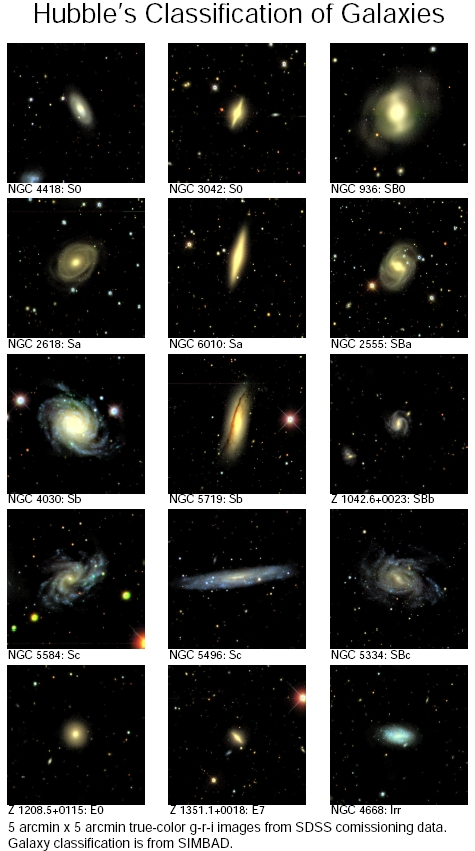
\includegraphics{figures/HubbleSDSS.jpg}}
\end{center}
\end{minipage}

\begin{minipage}[t]{15cm}
\begin{center}
\vskip -1in
{\large \color{red} Galaxies }
\end{center}

\begin{itemize}
\item
Galaxies are (mostly) made of stars (also gas, dust, active galactic nuclei -- AGN); 
hence have similar (but not identical!) color distributions
\item
They come in various shapes and forms (spiral vs. ellipticals; aka exponential
vs. de Vaucouleurs profiles)
\item
Some host AGNs, some have high star-formation rates, some are very unusual
(dwarf galaxies, mergers, etc.)
\item
We are interested in various distribution functions (e.g. for 
luminosity, colors, mass, age, metallicity, size, etc.) -- the hope is to
figure out {\color{blue} how galaxies formed and evolved}
\item
Nearest neighbors: the Andromeda galaxy (M31), Large and Small Magellanic Clouds, 
the Sgr Dwarf (may be more)
\end{itemize}  

\end{minipage}}
\vfill 
\end{slide}
%------------------------------------------------------------------------------


\begin{slide}
\begin{center}
{\large \color{red} 
                                The Basics of Basics
}
\end{center}


{\color{blue} Assumed that you are all familiar with these terms:}

\begin{itemize}
\item {\color{blue}general:} distance modulus, absolute magnitude, 
                             bolometric luminosity, the Planck function
\item {\color{blue}types of stars:} white dwarfs, horizontal branch, 
                           red giants, supergiants, subgiants, subdwarfs, etc.
\item {\color{blue}stellar properties:} effective temperature, spectral class, 
                           metalicity, mass, age 
\end{itemize}     
     
\vfill
\end{slide}


%------------------------------------------------------------------------------

\begin{slide}
\begin{center}
{\large \color{red} 
                                      Outline
}
\end{center}

\begin{enumerate}
\item {\color{blue} What do we observe:} a summary of the measurement process
\item {\color{blue} Hertzsprung-Russell Diagram:} a summary of gas ball physics
\item {\color{blue} Stellar parameters:} (mass, age, chemical composition) vs. 
(temperature, surface gravity, metalicity)
\item {\color{blue} Population Synthesis:} cooking up a galaxy
\item {\color{blue} Virial Theorem:} very brief intro to a very useful tool
\item {\color{blue} Open and Globular clusters:} simple stellar populations 
\end{enumerate}          
\vfill
\end{slide}




%------------------------------------------------------------------------------
\begin{slide}
\begin{center}
\bfseries
{\large {\color{red} What do we measure? \color{blue} Radiation Intensity:}}
\end{center}
\vskip 0.6in

{\centerline {\Huge \bf {\color{blue} 
 $I_\nu (\lambda, \alpha, \delta, t, {\bf p})$ }}}

\begin{itemize}

\item $I_\nu$ - energy (or number of photons) / time / Hz/ solid angle 
\item $\lambda$ - $\gamma$-ray to radio, depending on resolution:
      spectroscopy, narrow-band photometry, broad-band photometry
\item $\alpha, \delta$ - direction (position on the sky); the resolution 
    around that direction splits sources into unresolved (point) and resolved;
    interferometry, adaptive optics,...
\item $t$ - static vs. variable universe, sampling rate,...
\item {\bf p} polarization
\end{itemize}
\end{slide}
 
%------------------------------------------------------------------------------



%------------------------------------------------------------------------------
\begin{slide}
\begin{center}
\bfseries
{\large {\color{red} Examples:}}
\end{center}

\vskip 0.6in

{\bf Imaging (photometry):}
\begin{equation}
  I_\nu^{band}(<\alpha>, <\delta>, <t>) = \int_{0}^{\infty} S(\lambda)d\lambda 
\int_{0}^T dt \int_{\theta}d\Omega  \, I_\nu (\lambda, \alpha, \delta, t, {\bf p}) 
\end{equation}

{\color{red} SDSS: \color{blue} T = 54.1 sec, $\theta \sim$1.5 arcsec, filter width $\sim$1000 \AA}

{\bf Spectroscopy:}
\begin{equation}
  F_{\nu}^{object}(\lambda, <t>) = \int_{0}^{\infty} R(\lambda)d\lambda 
\int_{0}^T dt \int_{A}d\Omega  \, I_\nu (\lambda, \alpha_0, \delta_0, t, {\bf p}) 
\end{equation}

{\color{red} SDSS: \color{blue} T = 45 min, A: 3 arcsec fibers ($\sim$6 kpc at the redshift of 0.1),
R$\sim$2 \AA \, ($\sim$70 km/s)}

\end{slide}
 
%------------------------------------------------------------------------------


\picslide{SDSS2MASSfilters}{pdf}{SDSS and 2MASS photometric bandpasses}{1.2}{7}{-0.7}{3.5} 




%------------------------------------------------------------------------------
\begin{slide}
\begin{center}
\bfseries
{\large {\color{red} An example: SDSS photometry}}
\end{center}
\vskip 0.6in

\begin{itemize}
\item {\color{blue} Magnitudes:} there are five different types! Aperture,
         fiber, psf, model and Petrosian magnitudes.   
 \item {\color{blue} Radial Profiles:} all magnitudes are measured 
        using circularized brightness profiles extracted for a predefined 
        set of radii
\item {\color{red} Do we really need all these magnitudes?} 
\end{itemize}

\end{slide}
 
%------------------------------------------------------------------------------





%------------------------------------------------------------------------------
\begin{slide}
\begin{center}
\bfseries
{\large {\color{red} SDSS photometry}}
\end{center}
\vskip 0.6in

\begin{itemize}
\item {\color{blue} Magnitudes:} we need different magnitudes because, depending
     on an object's brightness profile, they have different noise properties
 \item {\color{blue} Unresolved sources:} {\color{red} aperture magnitudes} are the best, but 
       only for bright stars; for a given error, {\color{red} psf magnitudes} go 1-2 mags deeper; 
      {\color{red} fiber magnitudes} measure flux within 3 arcsec aperture, and thus estimate 
       the flux seen by spectroscopic fibers
\item {\color{blue} Resolved sources:} psf magnitudes don't include the total 
      flux, actually none of the various magnitudes includes the total flux
      for resolved sources! {\color{red} Petrosian magnitudes} include {\bf the same} 
      fraction of flux, independent of galaxy's angular size, however, they are
      very noisy for faint galaxies; {\color{red} model magnitudes} have smaller noise for
      faint galaxies (especially if you are interested only in colors)
\end{itemize}

\end{slide}
 
%------------------------------------------------------------------------------


%------------------------------------------------------------------------------
\begin{slide}
\begin{center}
\bfseries
{\large {\color{red} The count (uncalibrated flux) extraction}}
\end{center}
\vskip 0.6in

\begin{itemize}
\item {\color{blue} In the limit of a circular source, all fluxes (magnitudes) 
can be computed as:}

         $flux(type) \propto \int p(x) \, \Phi(x) \, 2\pi x \,dx$ 

\item {\color{blue} $type$:} aperture, fiber, psf, Petrosian, model
\item {\color{blue} $p(x)$:} circularized brightness profile
\item {\color{blue} $\Phi(x)$:} type-dependent weight function
\begin{itemize}
   \item {\color{red} aperture:} $\Phi(x)$ = 1 for $x<7.4$ arcsec, 0 otherwise
   \item {\color{red} fiber:} $\Phi(x)$ = 1 for $x<1.5$ arcsec, 0 otherwise
   \item {\color{red} psf:} $\Phi(x)$ = psf(x) for $x<3$ arcsec, 0 otherwise, 
               {\it photo} uses 2D integration (angle dependence)
   \item {\color{red} Petrosian:} $\Phi(x)$ = 1 for $x<R$ arcsec, 0 otherwise,
      $R$ depends on the measured galaxy profile: defined by the 
      ratio of the local surface brightness to the mean surface
      brightness within the same radius  
   \item {\color{red} model:} $\Phi(x)$ from a best-fit (deV or exp) 3-parameter 
     pre-computed profile (convolved with seeing); must be 2D integration
\end{itemize}

For {\color{red} signal-to-noise calculation}, see document {\bf An LSST document on astronomical 
signal-to-noise calculation and flux extraction} linked to the class webpage. 

More information about {\color{red} SDSS galaxy photometry} can be found in Strauss et al. (2002, AJ 124, 1810). 

\end{itemize} 

\end{slide}
 
%------------------------------------------------------------------------------


%------------------------------------------------------------------------------
\begin{slide}
\begin{center}
\bfseries
{\large {\color{red} Calibrated flux and magnitudes}}
\end{center}
\vskip 0.6in

\begin{itemize}
\item 
Given a specific flux of an object {\it at the top} of the atmosphere, 
$F_\nu(\lambda)$, a broad-band photometric system measures the in-band flux
\begin{equation}
\label{Fb}
           F_b = \int_0^\infty {F_\nu(\lambda) \phi_b(\lambda) d\lambda},
\end{equation}
where $\phi_b(\lambda)$ is the normalized system response for a given 
band (e.g. for SDSS $b=ugriz$)
\begin{equation}
\label{PhiDef}
\phi_b(\lambda) = {\lambda^{-1} S_b(\lambda) \over \int_0^\infty {\lambda^{-1} S_b(\lambda) d\lambda}}.
\end{equation}
\item
The overall atmosphere + system throughput, $S_b(\lambda)$, is obtained from  
\begin{equation}
\label{SDef}
         S_b(\lambda) = S^{atm}(\lambda) \times S_b^{sys}(\lambda). 
\end{equation}
\end{itemize} 

\end{slide}
 
%------------------------------------------------------------------------------

%------------------------------------------------------------------------------
% TWO-SIDED PAGE 
\begin{slide}

\hbox to \hsize{
\begin{minipage}[t]{10cm}
\begin{center}
\vskip -1.8in
\scalebox{1.0}{\hskip -1.7in 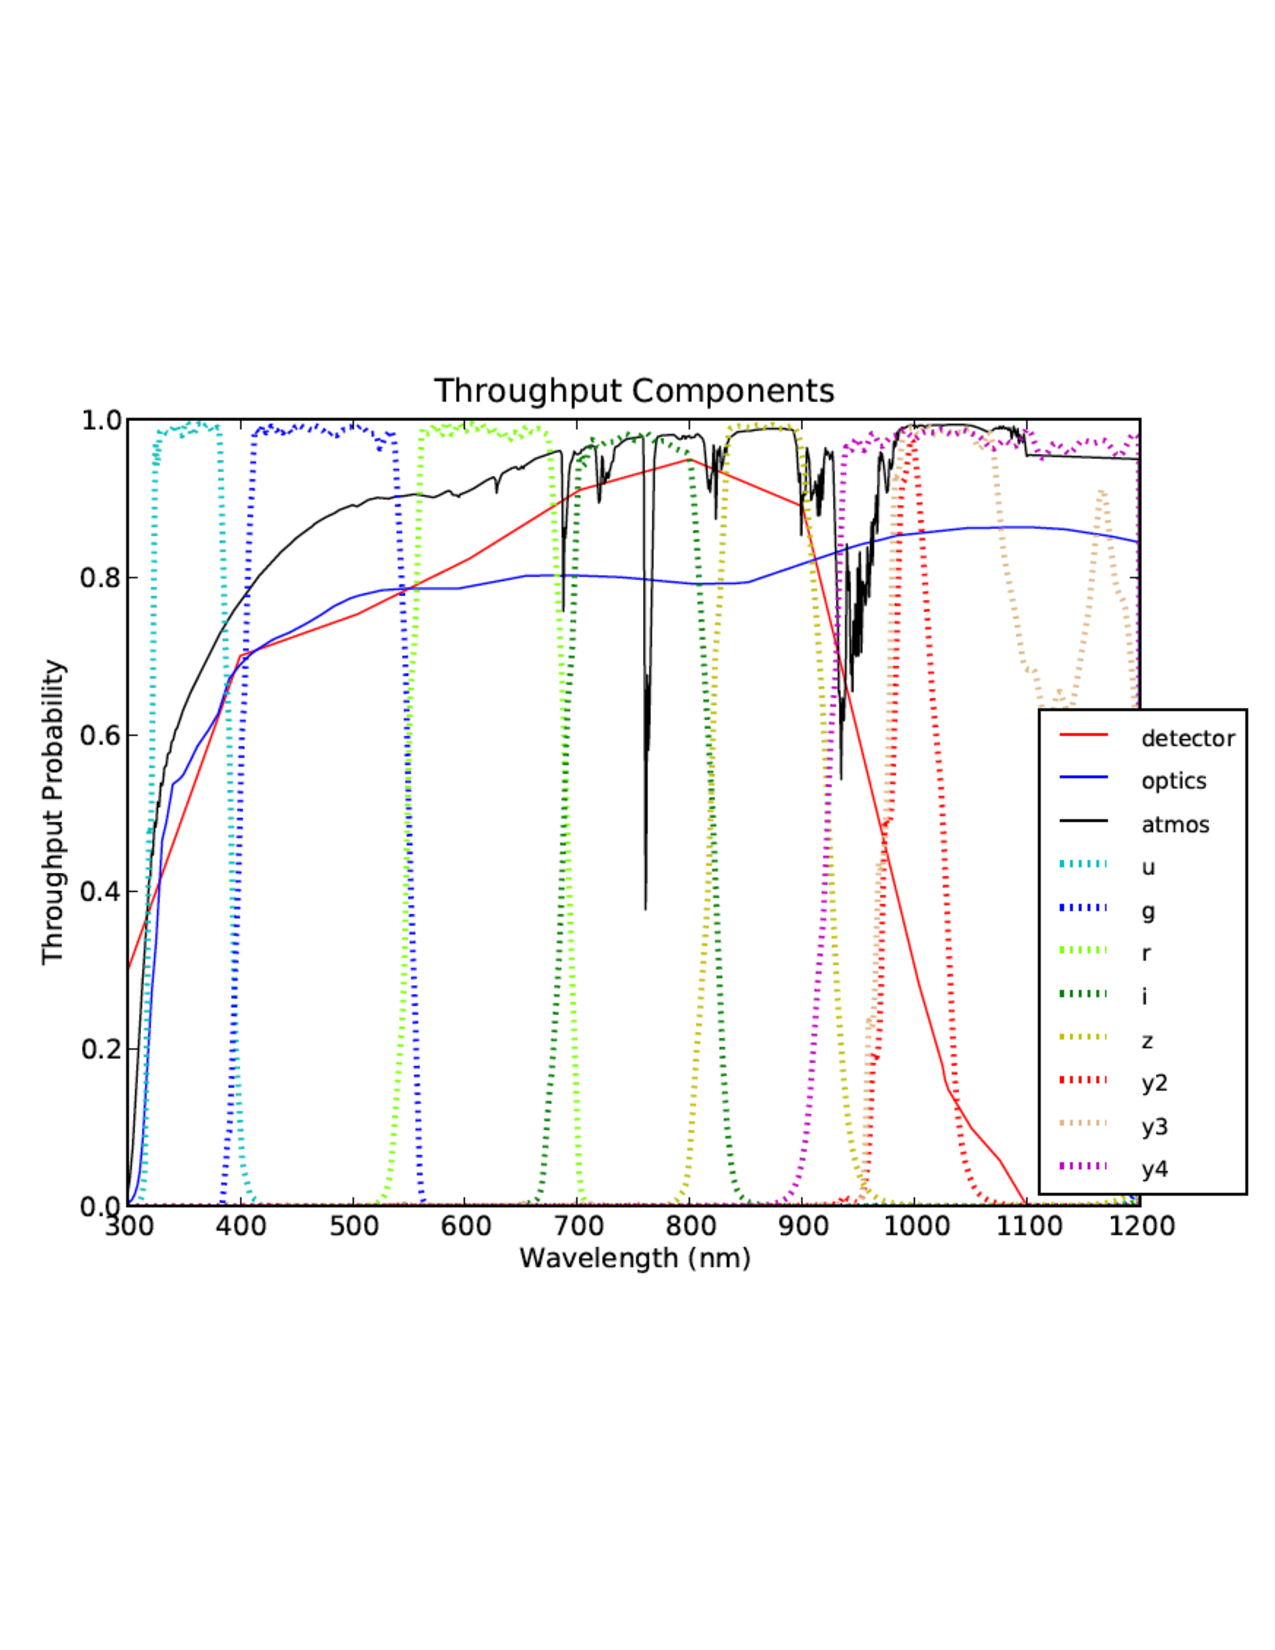
\includegraphics{figures/LSSTthroughput.pdf}}
\end{center}
\end{minipage}

\begin{minipage}[t]{8cm}
\begin{center}
{\large \color{red} LSST throughput}
\vskip -1in
\end{center}

\end{minipage}

}

\vfill 
\end{slide}
%--------------------------------------------------------------------------------------------


%------------------------------------------------------------------------------
% TWO-SIDED PAGE 
\begin{slide}

\hbox to \hsize{
\begin{minipage}[t]{10cm}
\begin{center}
\vskip -1.8in
\scalebox{1.0}{\hskip -1.7in 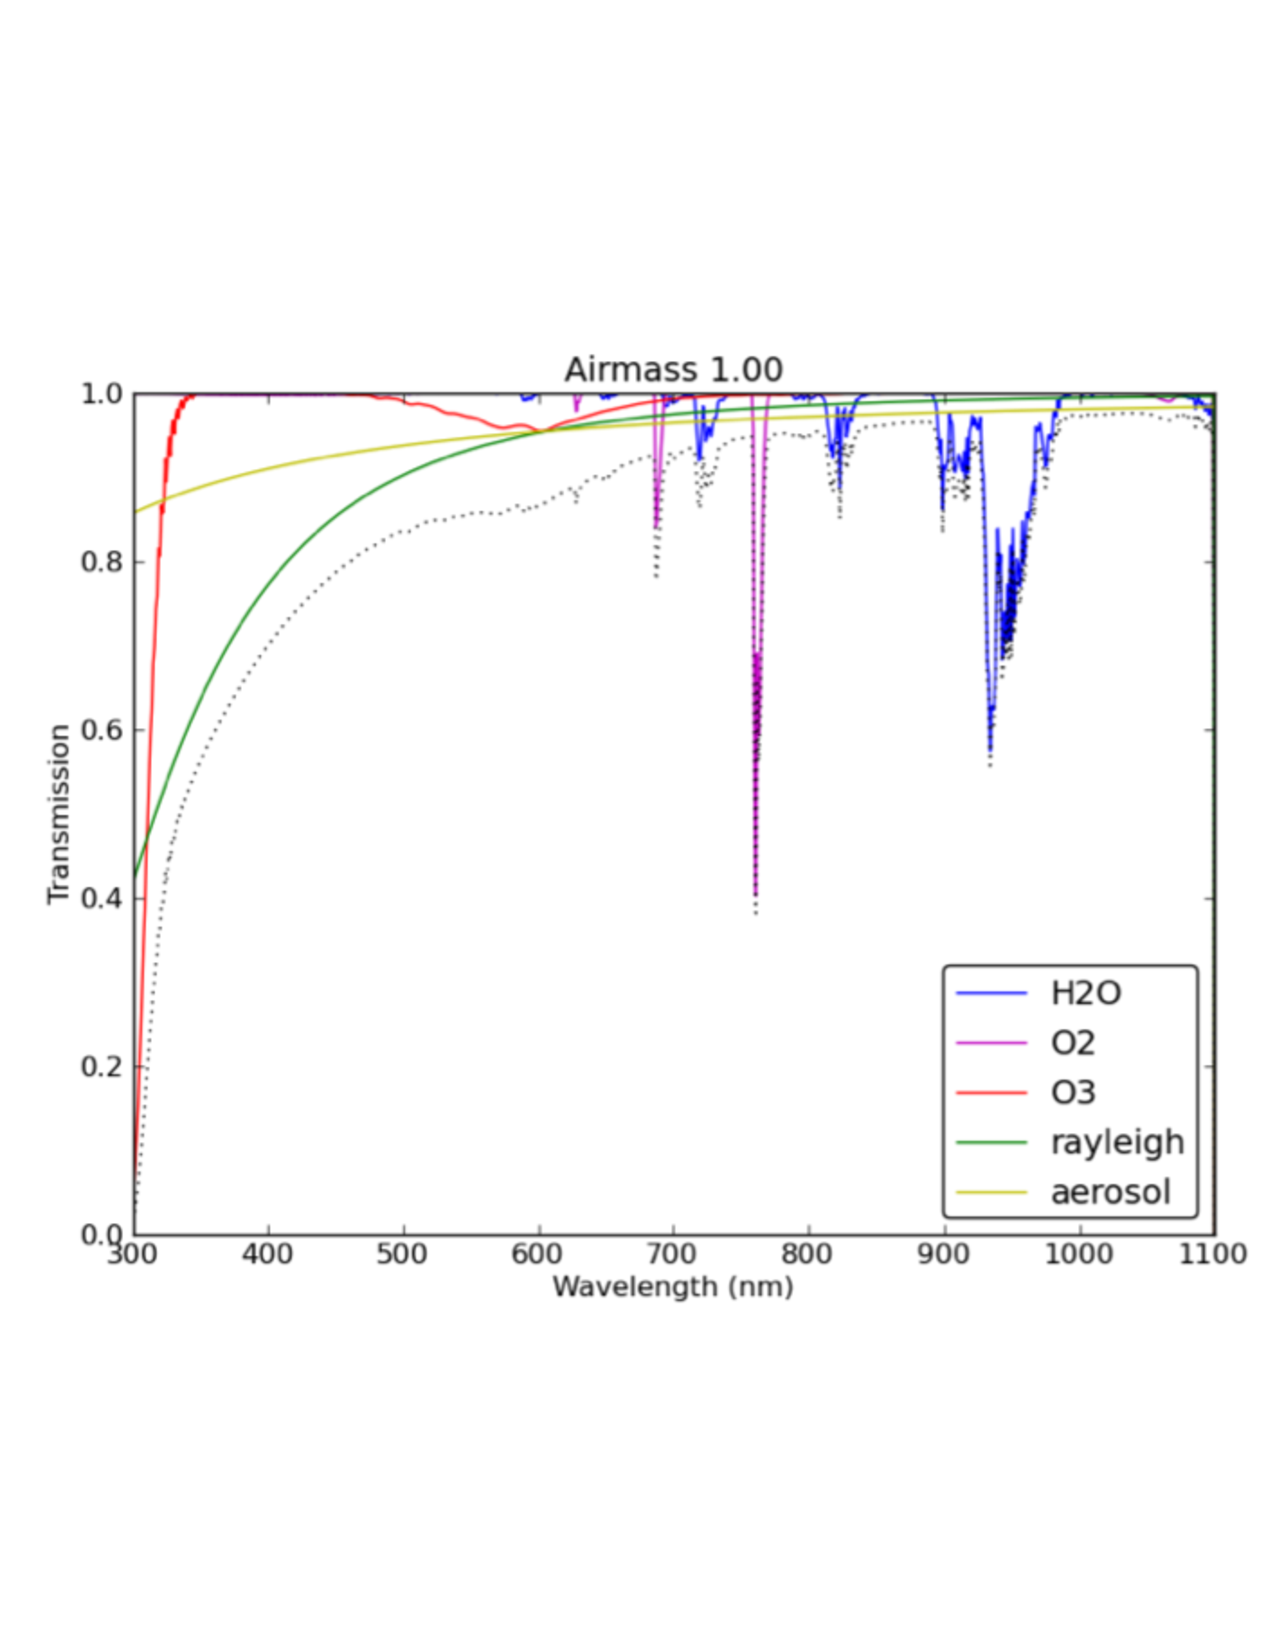
\includegraphics{figures/LSSTatmo.pdf}}
\end{center}
\end{minipage}

\begin{minipage}[t]{8cm}
\begin{center}
{\large \color{red} Atmosphere}
\vskip -1in
\end{center}

\end{minipage}

}

\vfill 
\end{slide}
%--------------------------------------------------------------------------------------------



%------------------------------------------------------------------------------
\begin{slide}
\begin{center}
\bfseries
{\large {\color{red} Calibrated flux and magnitudes}}
\end{center}
\vskip 0.6in

\begin{itemize}
\item
Photometric measurements are fully described by $F_b$ and its corresponding 
$\phi_b(\lambda)$. The relevant temporal, spatial and wavelength scales 
on which $\phi_b(\lambda)$ is known determine photometric accuracy.
Typically, it is assumed that $\phi_b(\lambda)$ ``defines'' a photometric
system (e.g. Johnson, Str\"omgren, SDSS)
\item
Traditionally, the in-band flux is reported on a magnitude scale
\begin{equation}
\label{ABmag}
                m_b = -2.5\log_{10}\left({F_b \over F_{AB} }\right).
\end{equation}
where $F_{AB} = 3631$ Jy (1 Jansky = 10$^{-26}$ W Hz$^{-1}$ m$^{-2}$ 
= 10$^{-23}$ erg s$^{-1}$ Hz$^{-1}$ cm$^{-2}$) is the flux normalization 
for AB magnitudes (Oke \& Gunn 1983). These magnitudes are also called 
``flat'' because for a source with ``flat'' spectral energy distribution 
(SED) $F_\nu(\lambda)= F_0$, $F_b = F_0$. 
\item
Note: it might be a bit confusing that $F_\nu(\lambda)$ is integrated over
wavelength in eq.~\ref{Fb}, and yet the result, $F_b$, has the same
units as $F_\nu(\lambda)$. This happens because the product 
$\phi_b(\lambda) d\lambda$ is dimensionless, and eq.~\ref{Fb} 
formally represents weighting of $F_\nu(\lambda)$ rather than 
its area integral. Of course, this is a consequence of the definition
of AB system\footnote{The fact that $F_\nu(\lambda)$ is multiplied by 
$S_b(\lambda)/\lambda$ and then integrated over wavelength is a 
consequence of the fact that CCDs are photon-counting devices. That is,
the units for $F_b$ are {\bf not} arbitrary. For more details, see 
Maiz Apell\'{a}niz 2006 (AJ 131, 1184).} 
in terms of $F_\nu(\lambda)$.  
\end{itemize} 

\end{slide}
 
%------------------------------------------------------------------------------

\picslide{SDSS2MASSfilters}{pdf}{SDSS and 2MASS photometric bandpasses}{1.2}{7}{-0.7}{3.5} 



%------------------------------------------------------------------------------
% TWO-SIDED PAGE 
\begin{slide}

\hbox to \hsize{
\begin{minipage}[t]{13cm}
\begin{center}
\vskip -0.8in
\scalebox{0.8}{\hskip -1.3in 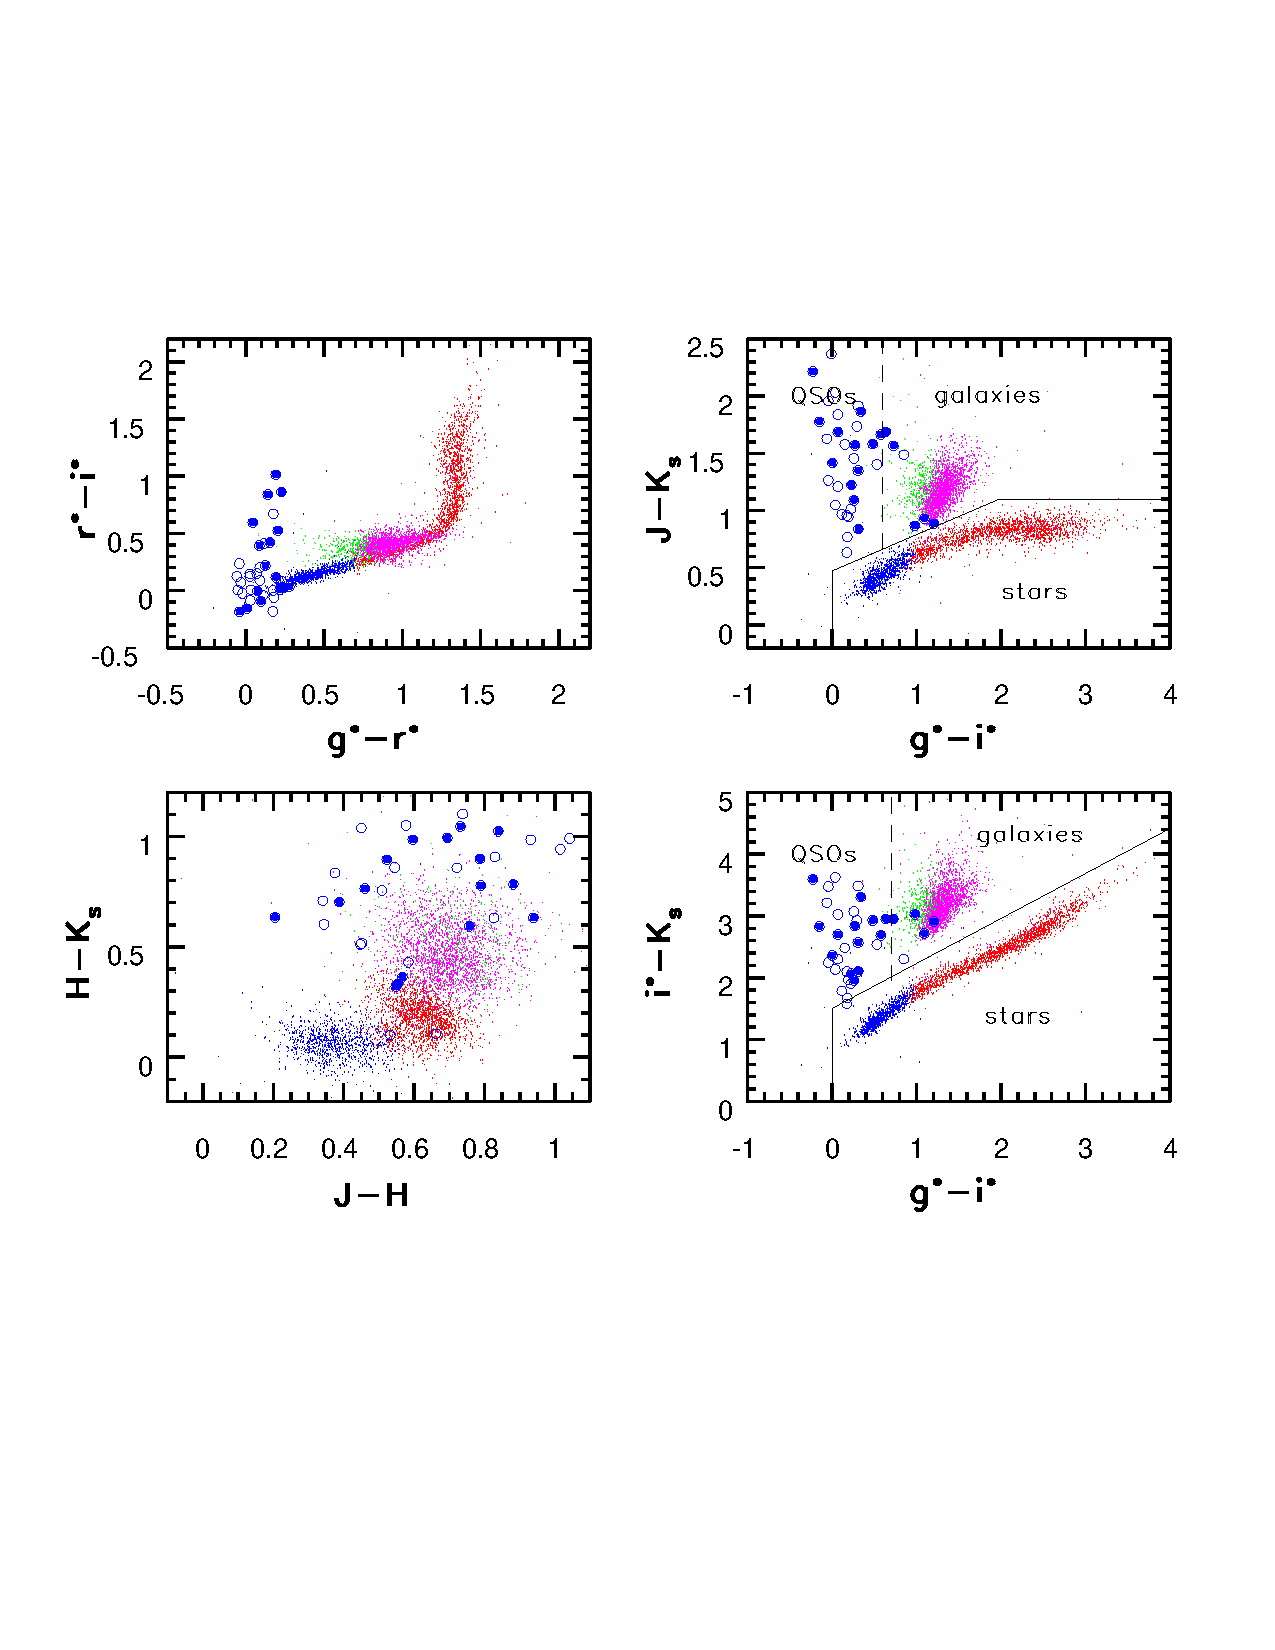
\includegraphics{figures/SDSSMASSccd.pdf}}
\end{center}
\end{minipage}


\begin{minipage}[t]{11cm}
\begin{center}
{\large \color{red} SDSS-2MASS sources}
\end{center}

\begin{itemize} 
\item
Blue/red: blue and red stars; green/magenta: blue and red galaxies,
Circles: quasars ($z<2.5$)
\item
Optical/IR colors allow an efficient star-quasar-galaxy separation
\item
8-band accurate and robust photometry excellent for finding
objects with atypical SEDs (e.g. red AGNs, L/T dwarfs, binary
stars)
\end{itemize} 

\end{minipage}}
\vfill 
\end{slide}


%------------------------------------------------------------------------------
% TWO-SIDED PAGE 
\begin{slide}

\hbox to \hsize{
\begin{minipage}[t]{12cm}
\begin{center}
\vskip -0.6in
\scalebox{0.45}{\hskip -1.0in 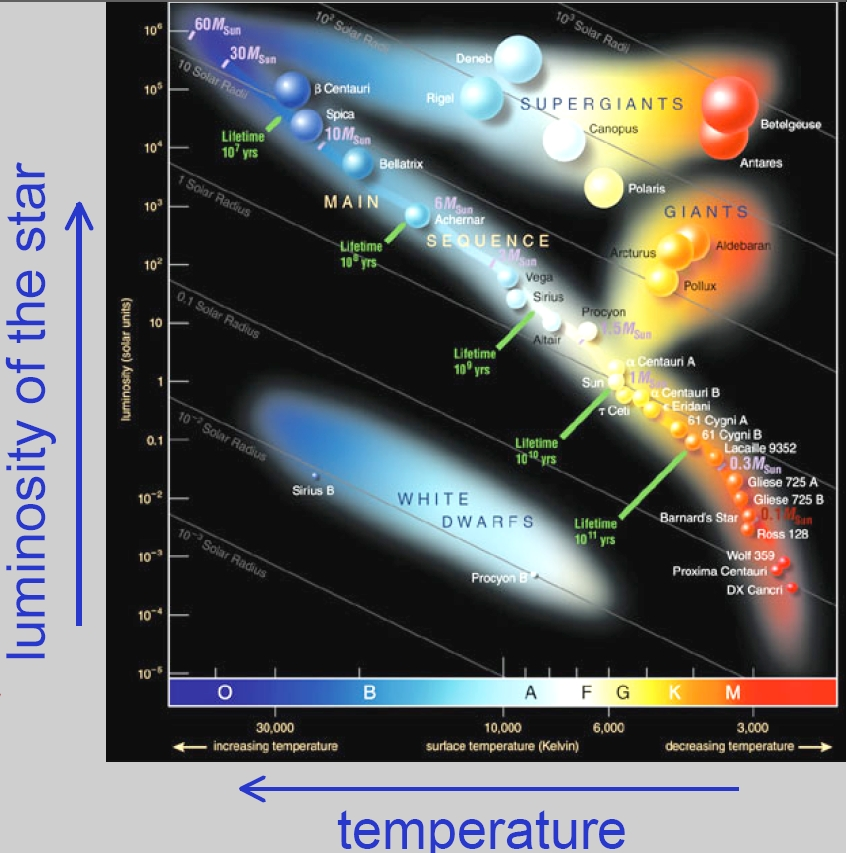
\includegraphics{figures/HR.jpg}}
\vskip 0.1in
\scalebox{0.4}{\hskip  -8.5in 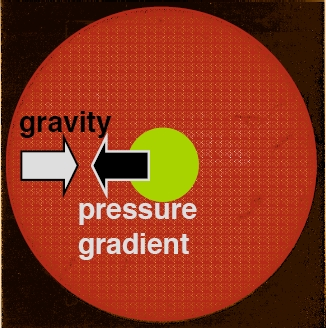
\includegraphics{figures/2forces.jpg}}
\vskip -1.9in
\scalebox{0.25}{\hskip  8.5in 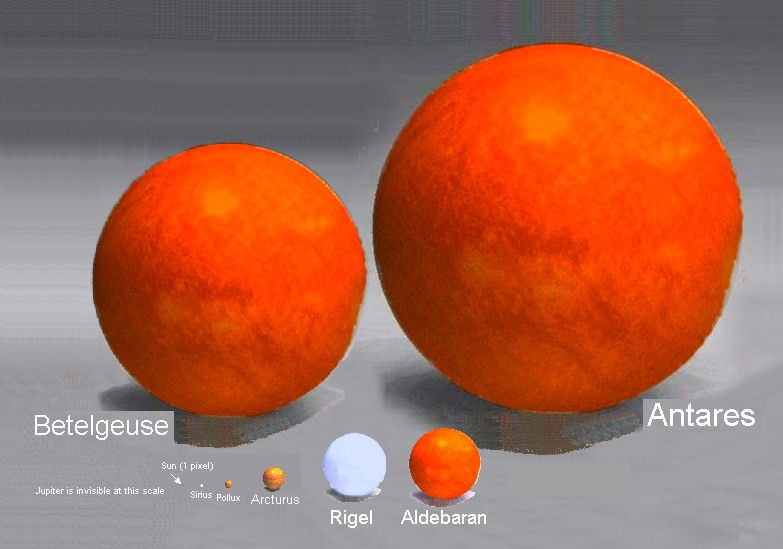
\includegraphics{figures/pic29691.jpg}}
\vskip -1.1in
\scalebox{0.25}{\hskip 22.5in 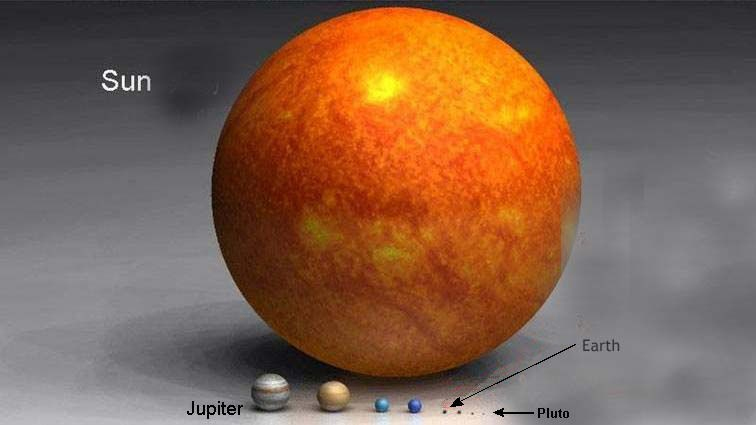
\includegraphics{figures/pic35878.jpg}}
\vskip -0.4in
\end{center}
\vskip -0.5in
Check out HR simulator at
\begin{verbatim}
http://www.astro.ubc.ca/~scharein/a311/Sim/hr/HRdiagram.html
\end{verbatim}
\end{minipage}

\begin{minipage}[t]{12cm}
\begin{center}
\phantom{xxx}
\vskip -1in
{\large \color{red} Hertzsprung-Russell Diagram }
\end{center}


\begin{itemize}
\item {\color{blue} Stars are balls of hot gas} in hydrodynamical and thermodynamical equilibrium
\item {\color{blue} Equilibrium based on two forces}, gravity: inward, radiation pressure: outward
\item {\color{blue} Temperature and size} cannot take arbitrary values: the allowed ones are 
     summarized in HR diagram 
\item {\color{red} $L = {\rm Area} \, {\rm  x} \, {\rm  Flux} = 4\pi R^2 \sigma T^4$}
\item {\color{blue} Luminosity and size} span a {\bf huge} dynamic range!
\end{itemize}

\end{minipage}}
\vfill 
\end{slide}
%--------------------------------------------------------------------------------------------


%------------------------------------------------------------------------------
% TWO-SIDED PAGE 
\begin{slide}

\hbox to \hsize{
\begin{minipage}[t]{12cm}
\begin{center}
\vskip -0.8in
\scalebox{0.75}{\hskip -1.4in 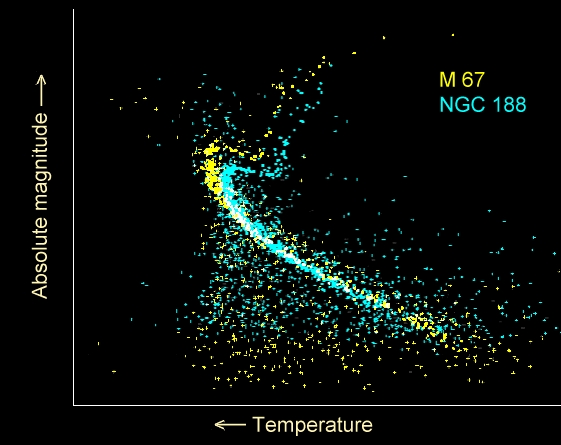
\includegraphics{figures/HR_ages.jpg}}
%\vskip -0.007in
\scalebox{0.55}{\hskip -1.8in 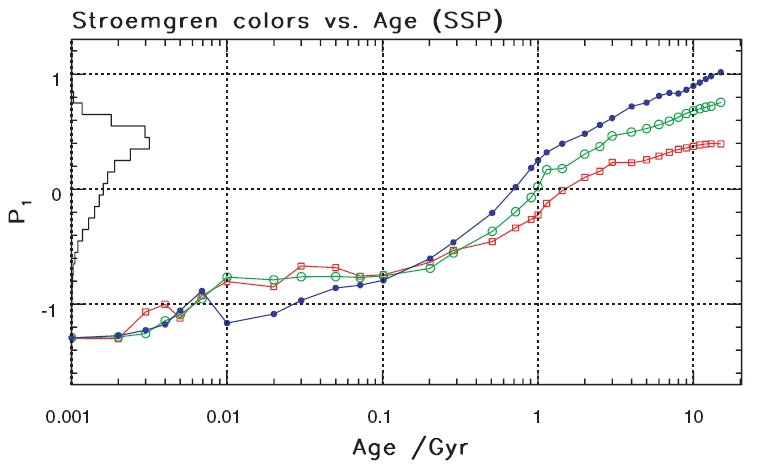
\includegraphics{figures/Smolcic_fig8a.jpg}}

\end{center}
\end{minipage}

\begin{minipage}[t]{12cm}
\begin{center}
\vskip -1in
{\large \color{red} HR Diagram: Stellar Age }
\end{center}


\begin{itemize}
\item {\color{blue} The main sequence} is where most of lifetime is spent.
\item {\color{blue} The position on the main sequence} is determined by mass! 
\item {\color{blue} The lifetime depends on mass:} massive (hot and blue) stars
                    have {\bf much} shorter lifetimes than red stars
\item {\color{blue} After a burst of star formation,} blue stars disappear 
                    {\bf very quickly}, $10^8$ years or so
\item {\color{blue} Galaxies are made of stars:} if there is no ongoing 
         star formation, they are red; if blue, there {\bf must} be actively
         making stars!
\item Turn-off color depends on both age and metallicity (later...) 
\end{itemize}

\end{minipage}}
\vfill 
\end{slide}
%--------------------------------------------------------------------------------------------



%------------------------------------------------------------------------------
% TWO-SIDED PAGE 
\begin{slide}

\hbox to \hsize{
\begin{minipage}[t]{12cm}
\begin{center}
\vskip -0.8in
\scalebox{0.55}{\hskip -1.4in 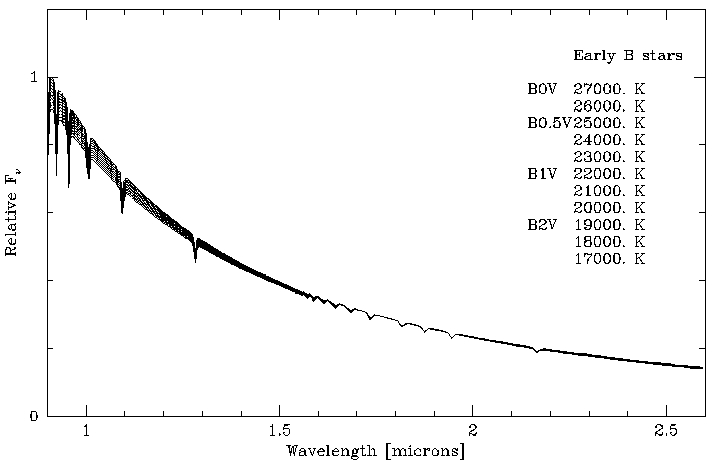
\includegraphics{figures/Kurucz_Bstars.jpg}}
%\vskip -0.007in
\scalebox{0.55}{\hskip -1.4in 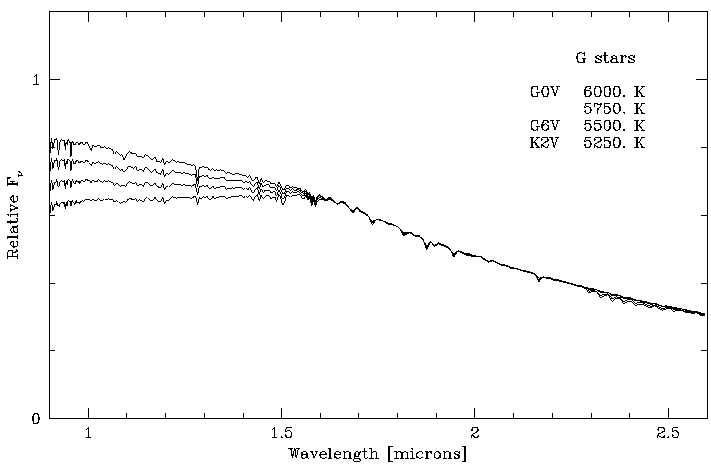
\includegraphics{figures/Kurucz_Gstars.jpg}}

\end{center}
\end{minipage}

\begin{minipage}[t]{12cm}
\begin{center}
\vskip -1in
{\large \color{red} Stellar Parameters }
\vskip -1in
\end{center}


\begin{itemize}
\item {\color{blue} The stellar spectral energy distribution} is a function of 
      mass, chemical composition and age, a theorist would say
\item {\color{blue} The stellar spectral energy distribution} is a function of 
      effective temperature, surface gravity and metallicity (at the accuracy 
      level of 1\%); the first two simply describe the position in the HR diagram
\item {\color{blue} Kurucz models (1979)} describe SEDs of (not too cold) main
        sequence stars, as a function of $T_{\rm eff}$, $log(g)$ and $[Fe/H]$
\end{itemize}

\end{minipage}}
\vfill 
\end{slide}
%--------------------------------------------------------------------------------------------




%------------------------------------------------------------------------------
% TWO-SIDED PAGE 
\begin{slide}

\hbox to \hsize{
\begin{minipage}[t]{12cm}
\begin{center}
\vskip -0.8in
\scalebox{0.55}{\hskip -1.7in 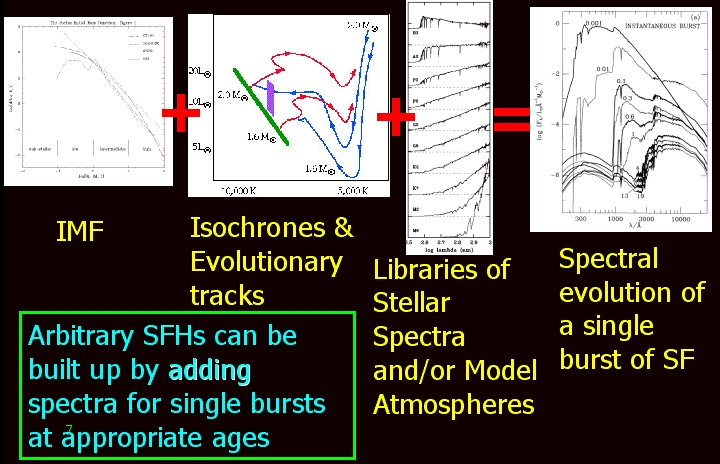
\includegraphics{figures/popSynth_JD.jpg}}
%\vskip -0.007in
\scalebox{0.75}{\hskip -1.4in 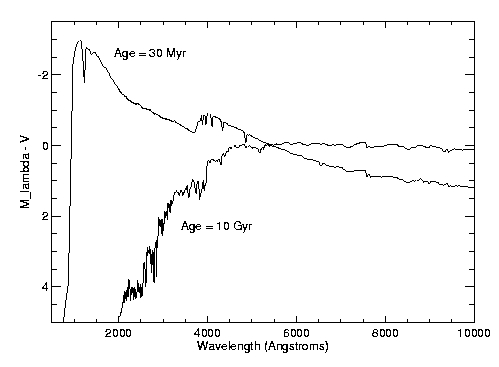
\includegraphics{figures/BC-youngold-SED-mor99.jpg}}

\end{center}
\end{minipage}

\begin{minipage}[t]{12cm}
\begin{center}
\vskip -1in
{\large \color{red} Population Synthesis: modeling SEDs of galaxies }
\end{center}


\begin{enumerate}
\item {\color{blue} A burst of star formation:} a bunch of stars (i.e. our galaxy) 
      was formed some time ago: {\bf age}
\item {\color{blue} The mass distribution} of these stars is given by a function called
        {\bf initial mass function, IMF}, roughly a power-law $n(M) \propto M^{-3}$
\item {\color{blue} The stellar distribution in the HR diagram} is given by the adopted
      age and IMF; equivalently, can adopt a CMD for a globular or open cluster; assume
      {\bf metallicity} and get a model (i.e. stellar SED, e.g. from Kurucz) for each 
      star and add them up
\end{enumerate}

\end{minipage}}
\vfill 
\end{slide}
%--------------------------------------------------------------------------------------------


%------------------------------------------------------------------------------
% TWO-SIDED PAGE 
\begin{slide}

\hbox to \hsize{
\begin{minipage}[t]{13cm}
\begin{center}
\vskip -0.8in
\scalebox{0.55}{\hskip -1.7in 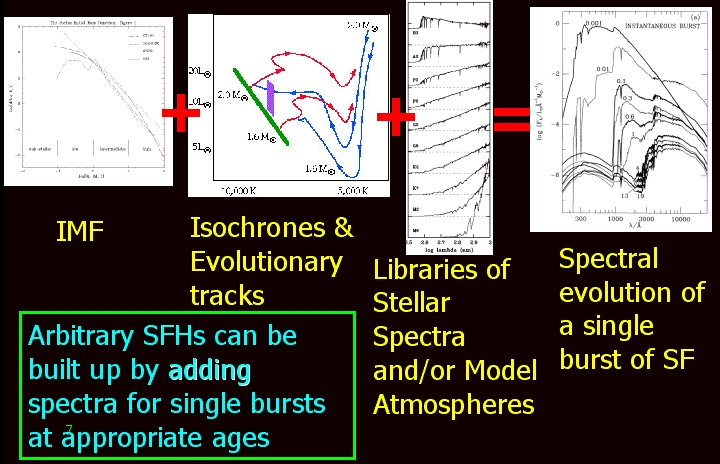
\includegraphics{figures/popSynth_JD.jpg}}
\vskip 0.4in
\scalebox{0.65}{\hskip -5.8in 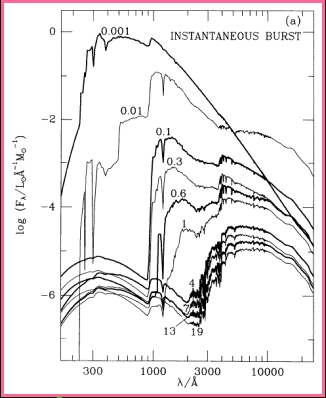
\includegraphics{figures/popSynth_burst.jpg}}
\vskip -3.6in
\scalebox{0.65}{\hskip  3.4in 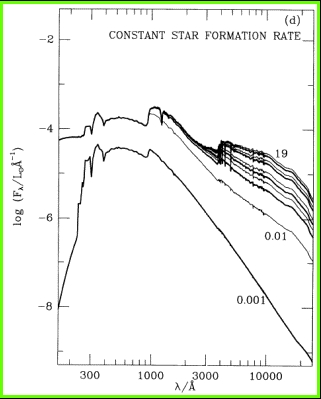
\includegraphics{figures/popSynth_const.jpg}}

\end{center}
\end{minipage}

\begin{minipage}[t]{11cm}
\begin{center}
\vskip -1in
{\large \color{red} Population Synthesis: modeling SED of galaxies }
\end{center}


\begin{enumerate}
\item {\color{blue} A burst of star formation:} {\bf age}
\item {\color{blue} The initial mass function, IMF}
\item {\color{blue} The stellar distribution in the HR diagram} and metallicity: {\bf add 
                    SEDs for all stars}, the result is
\item {\color{blue} Simple stellar population} as a function of {\bf age} and {\bf metallicity} 
\item {\color{blue} Star-formation history}, or the distribution of stellar ages,
      tells us how to combine such simple stellar populations to get SED of a realistic
      galaxy
\end{enumerate}

\end{minipage}}
\vfill 
\end{slide}
%----------------------------------------------------------------------------


\picslide{RvsBgalaxies_JDsummary}{jpg}{}{1.0}{7}{-0.5}{0.1}

%------------------------------------------------------------------------------










%------------------------------------------------------------------------------
% TWO-SIDED PAGE 
\begin{slide}

\hbox to \hsize{
\begin{minipage}[t]{9cm}
\begin{center}
\vskip -0.2in
\scalebox{0.8}{\hskip -1.3in 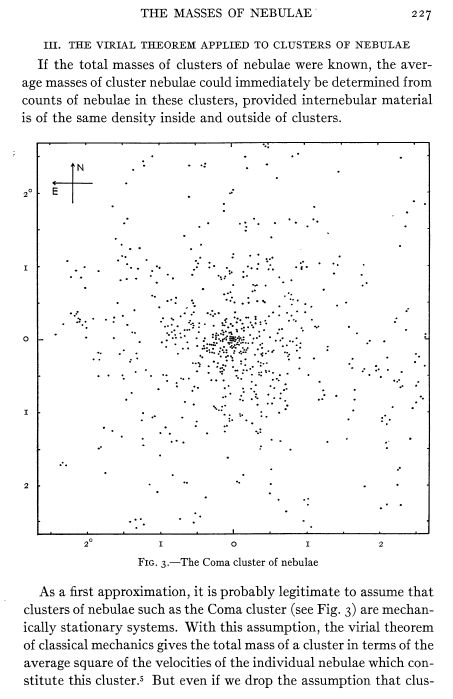
\includegraphics{figures/Zw1.jpg}}
\end{center}
\end{minipage}

\begin{minipage}[t]{13cm}
\begin{center}
\vskip -1in
{\large \color{red}  The Virial Theorem }
\end{center}

\begin{itemize}
\item In a system of N particles, gravitational forces tend to 
pull the system together and the stellar velocities tend to 
make it fly apart. It is possible to relate kinetic and potential
energy of a system through the change of its moment of intertia 
\item In a {\color{blue} steady-state system}, these tendencies
are balanced, which is expressed quantitatively through
the {\color{blue} the Virial Theorem}. 
\item {\color{blue} A system that is not in balance will tend to move
towards its virialized state.} 
\end{itemize}     

\end{minipage}}
\vfill 
\end{slide}
%------------------------------------------------------------------------------




%------------------------------------------------------------------------------
\begin{slide}
\begin{center}
{\large \color{red} 
                    The Scalar Virial Theorem}
\end{center}

The Virial Theorem will be discussed in detail later in this class.  For now, 
all we need to know is the final result for the {\color{blue} Scalar} Virial Theorem:
the {\it average} kinetic and potential energy must be in balance:
\eq{
             E = K + \Phi = -K = {1\over 2} \Phi
} 
where $K = M<v^2>/2$ is the kinetic energy, $\Phi$ is the gravitational potential
energy, and $E$ is the total energy (negative for a gravitationally bound system). 


\vfill
\end{slide}








%------------------------------------------------------------------------------
\begin{slide}
\begin{center}
\vskip 1.5in
\scalebox{5.1}{\hskip -0.1in 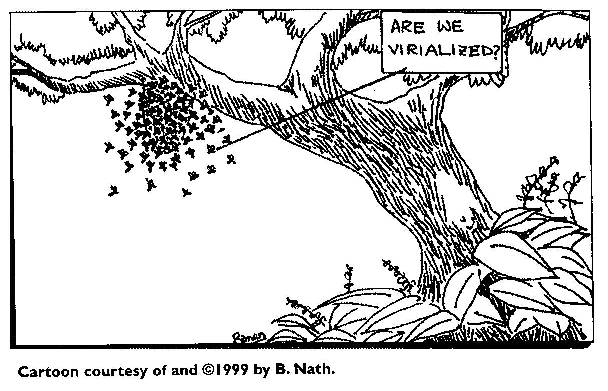
\includegraphics{figures/are_we_virialized.jpg}}
\end{center}

\vfill
\end{slide}




%------------------------------------------------------------------------------
\begin{slide}
\begin{center}
{\large \color{red} 
                    The Scalar Virial Theorem: Applications  }
\end{center}

\begin{itemize}
\item 
If a system collapses from infinity, half of the potential
energy will end up in kinetic energy, and the other half
will be disposed of! From the measurement of the circular
velocity and the mass of Milky Way (which constrain 
the kinetic energy), we conclude that during their formation,
galaxies radiate away about $3\times10^{-7}$ of their
rest-mass energy.
\item
For a virialized spherical system, $M = 2 R \sigma^2 / G$. 
We can estimate total mass from the size and velocity dispersion.
E.g. for a cluster with $\sigma$=12 km/s, and R=3 pc, 
we get $M = 2\times 10^5$ M$_\odot$ (note that $G=233$ in 
these units)
\item 
{\color{red} Think about this for the next time:} Evil aliens
give a ''kick'' to our Moon that increases its kinetic energy
by 10\%. What will happen with its orbit? 
\end{itemize}     

\vfill
\end{slide}




%------------------------------------------------------------------------------
% TWO-SIDED PAGE 
\begin{slide}

\hbox to \hsize{
\begin{minipage}[t]{9cm}
\begin{center}
\vskip -0.6in
\scalebox{0.45}{\hskip -1.7in 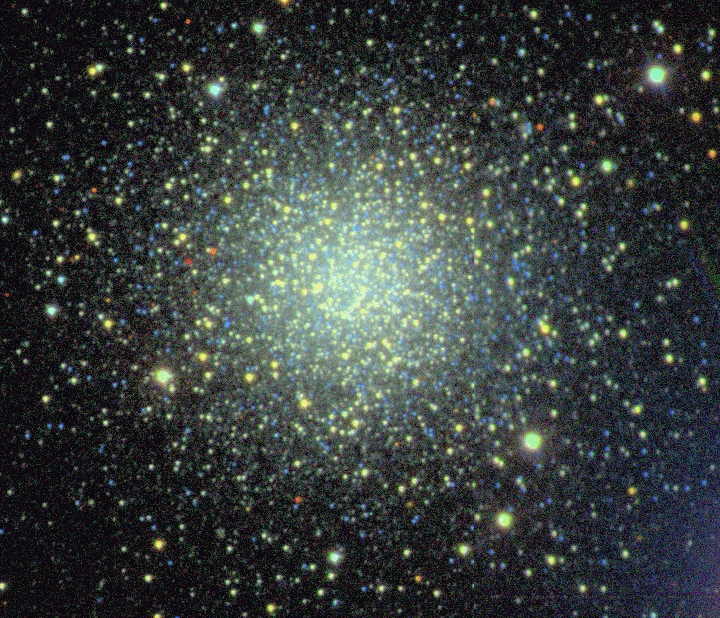
\includegraphics{figures/NGC2419-core.jpg}}
\vskip 0.1in
\scalebox{0.30}{\hskip -2.1in 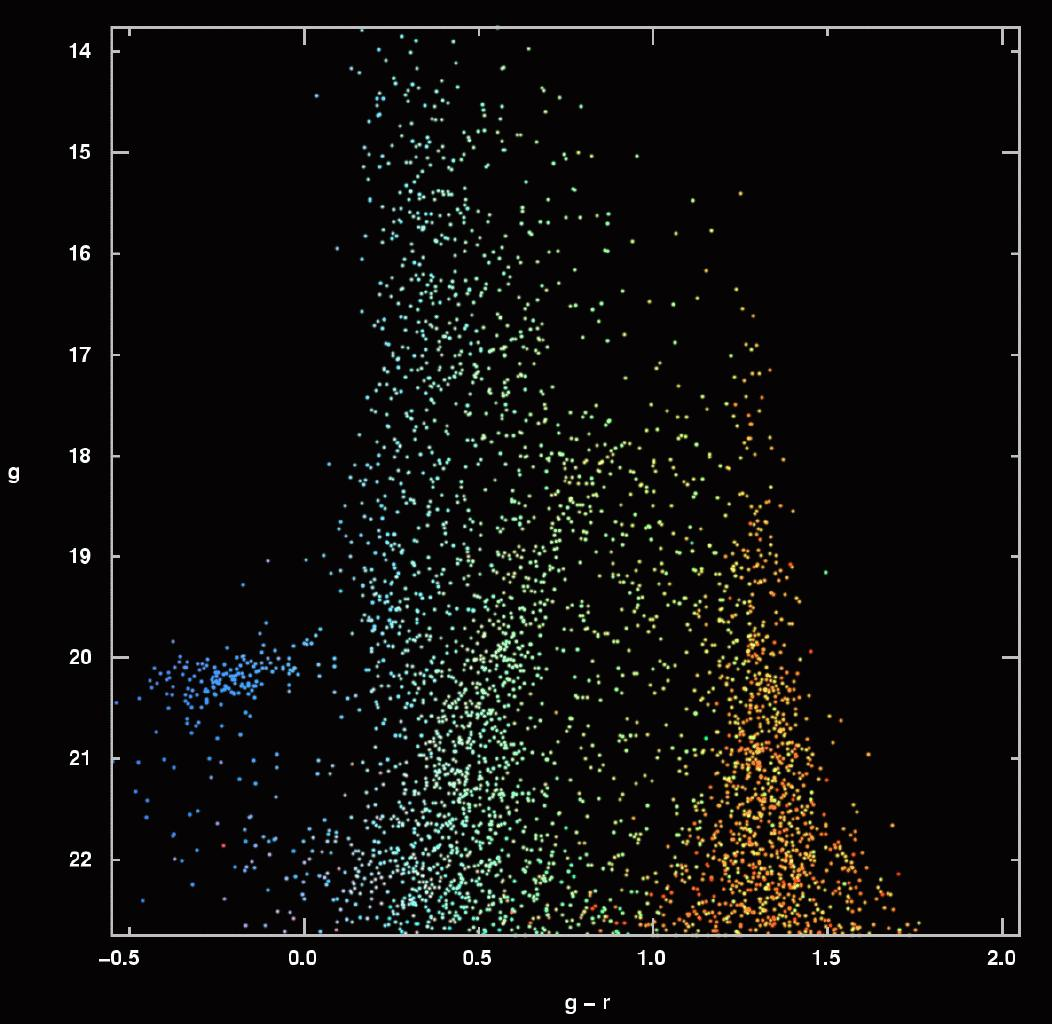
\includegraphics{figures/NGC2419-gr.jpg}}

\end{center}
\end{minipage}

\begin{minipage}[t]{15cm}
\begin{center}
\vskip -1in
{\large \color{red} Open and Globular Clusters}
\end{center}


\begin{itemize}
\item {\bf Top left:} SDSS gri composite image of globular cluster NGC 2419;
         note blue (literally) horizontal branch stars and yellowish (red)
         giants; the image is color-coded by the observed  g-r
\item {\bf Bottom left:} the SDSS g vs. g-r color-magnitude diagram of the area 
       surrounding NGC 2419; the dots are
       color-coded by the observed SDSS g-r color
       % note the close correspondence with the top panel!
\item {\bf Below:} the SDSS gri composite image of open cluster M67 (NGC 2682)
\end{itemize}
\vskip 0.0in
\scalebox{0.29}{\hskip 1.7in 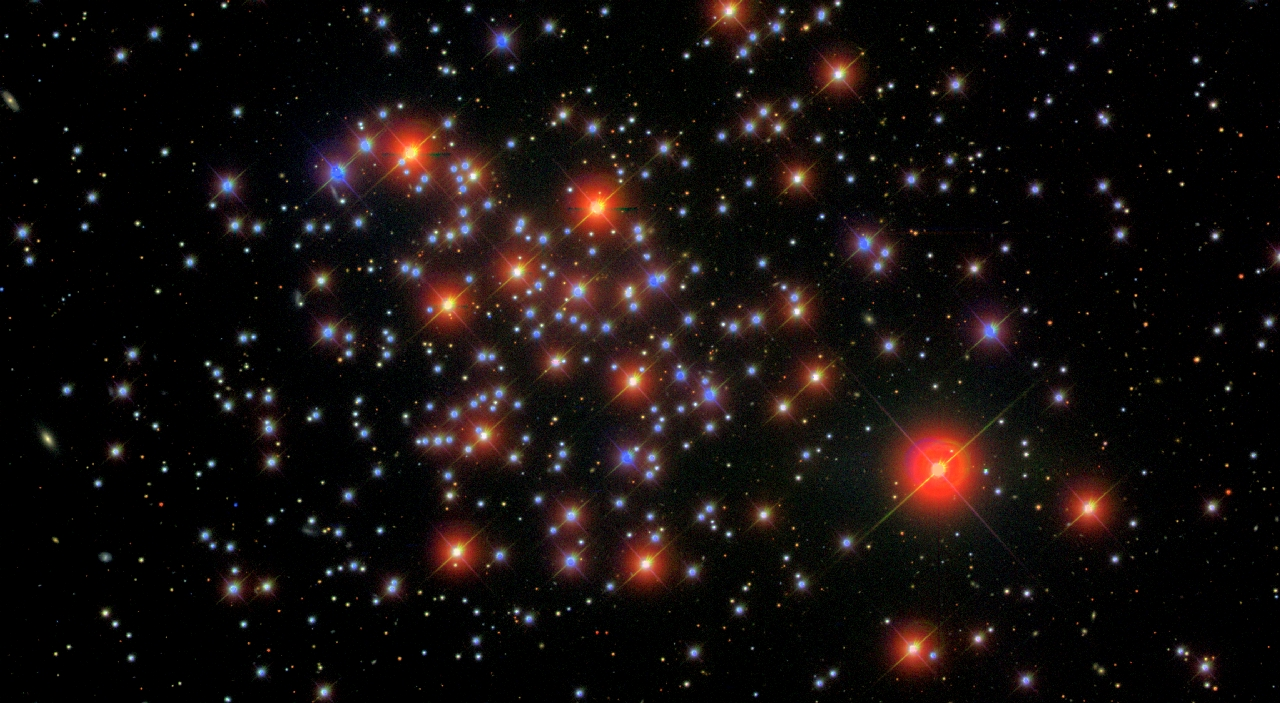
\includegraphics{figures/NGC2682.jpg}}

\end{minipage}}
\vfill 
\end{slide}
%--------------------------------------------------------------------------------------------


%------------------------------------------------------------------------------
% TWO-SIDED PAGE 
\begin{slide}

\hbox to \hsize{
\begin{minipage}[t]{12cm}
\begin{center}
\vskip -0.8in
\scalebox{0.75}{\hskip -1.4in 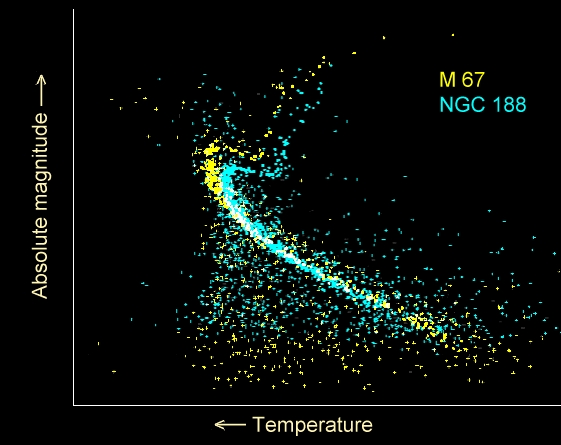
\includegraphics{figures/HR_ages.jpg}}
%\vskip -0.007in
\scalebox{0.55}{\hskip -1.8in 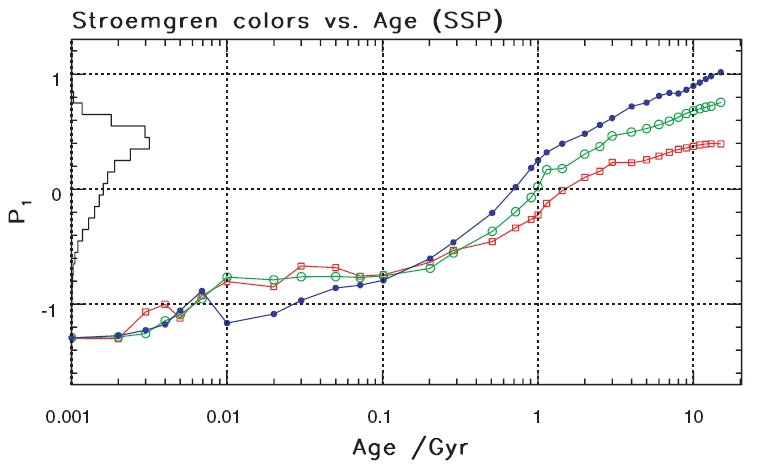
\includegraphics{figures/Smolcic_fig8a.jpg}}

\end{center}
\end{minipage}

\begin{minipage}[t]{12cm}
\begin{center}
\vskip -1in
{\large \color{red} Open and Globular Clusters}
\end{center}


\begin{itemize}
\item Stellar clusters are excellent probes of stellar astrophysics
\item {\color{blue} The three main advantages:} 
   \begin{enumerate}
      \item All stars at roughly the same distance
      \item All stars have roughly the same composition
      \item All stars have roughly the same age
   \end{enumerate}
\item The position of the main sequence, at a given color, 
       depends on metallicity 
\item The turn-off color depends on age and metallicity 
\item Other features, such as morphology of blue horizontal 
   branch and red giant branch, also depend on age and metallicity 

\end{itemize}

\end{minipage}}
\vfill 
\end{slide}
%--------------------------------------------------------------------------------------------




%------------------------------------------------------------------------------
% TWO-SIDED PAGE 
\begin{slide}

\hbox to \hsize{
\begin{minipage}[t]{11cm}
\begin{center}
\vskip -0.6in
\scalebox{1.0}{\hskip -0.7in 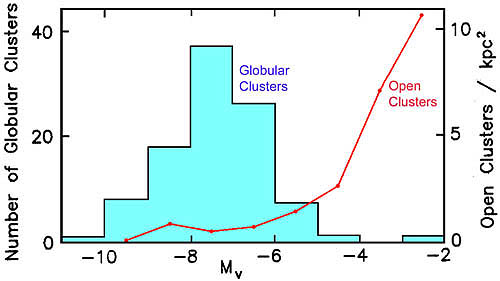
\includegraphics{figures/ClusterLumFn.jpg}}
\vskip 0.4in
\scalebox{0.5}{\hskip -1.7in 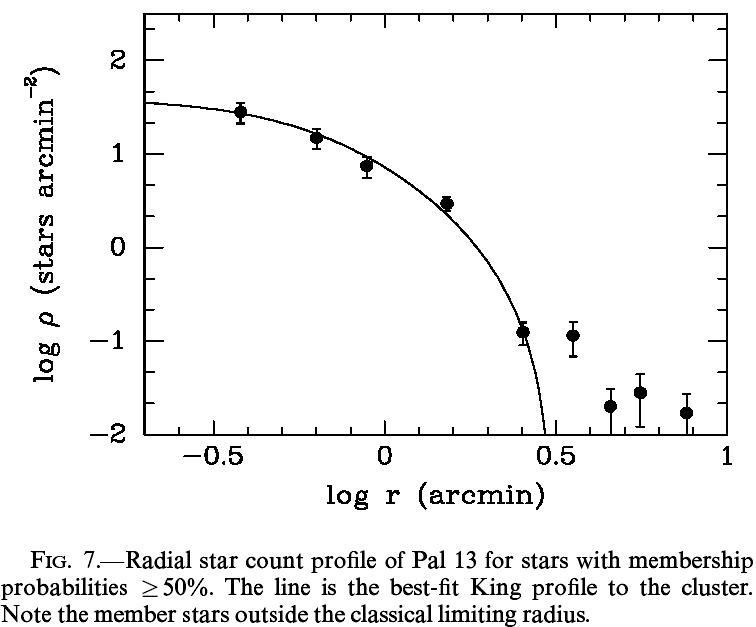
\includegraphics{figures/Pal13.jpg}}
\end{center}
\end{minipage}

\begin{minipage}[t]{13cm}
\begin{center}
\vskip -1in
{\large \color{red} Open and Globular Clusters}
\end{center}


\begin{itemize}
\item Open clusters are younger and concentrated towards the Galactic plane;
      globular clusters are more spherically distributed, at larger distances
      from the galactic center, have much lower metallicity and are much older
\item {\bf Top left:} luminosity functions for globular and open clusters 
       are very different 
\item {\bf Bottom left:} dying globular cluster Pal 13 (Siegel et al. 2001, 
      AJ 121, 935): Spatial profiles of globular clusters usually closely 
      follow King profiles (c.f. Tom's class on stellar dynamics);
      next slide stolen from Doug Heggie
\end{itemize}

\end{minipage}}
\vfill 
\end{slide}
%--------------------------------------------------------------------------------------------

\picslide{heggie1}{jpg}{UV-radio surveys}{0.92}{7}{-0.9}{3.5}

%------------------------------------------------------------------------------
% TWO-SIDED PAGE 
\begin{slide}

\hbox to \hsize{
\begin{minipage}[t]{11cm}
\begin{center}
\vskip -0.3in
\scalebox{1.05}{\hskip -0.9in 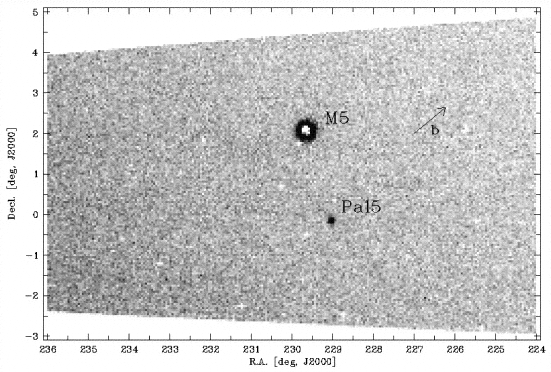
\includegraphics{figures/Pal5tailsRaw.jpg}}
%\vskip -0.007in
\vskip 0.3in
\scalebox{1.05}{\hskip -0.9in 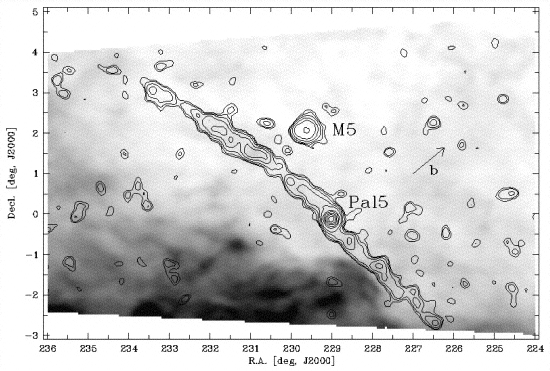
\includegraphics{figures/Pal5tails.jpg}}

\end{center}
\end{minipage}

\begin{minipage}[t]{13cm}
\begin{center}
\vskip -1in
{\large \color{red} Tidal Tails around Globular Clusters }
\end{center}


\begin{itemize}
\item {\bf Top left:} SDSS stellar counts around globular clusters 
             M5 and Pal5 
\item {\bf Bottom left:} matched filter extraction of tidal tails around
         Pal 5 (gray: SFD E(B-V)) by Rockosi et al. (2002) and
         Odenkirchen et al. (2003)
\item For more details about matched filter method, see Grillmair (2008,
       arXiv:0811.3965; and references therein)
\item {\color{blue} Tidal tails provide strong constraints on the Milky 
       Way gravitational potential.} 
\end{itemize}

\end{minipage}}
\vfill 
\end{slide}
%-----------------------------------------------------------------------------



\picslide{Pal5orbit}{jpg}{}{0.82}{7}{-0.9}{3.5}


	
\picslide{prfig4}{jpg}{}{0.82}{7}{0.0}{3.5}



%------------------------------------------------------------------------------
% TWO-SIDED PAGE 
\begin{slide}

\hbox to \hsize{
\begin{minipage}[t]{8cm}
\begin{center}
\vskip -0.8in
\scalebox{0.5}{\hskip -1.6in 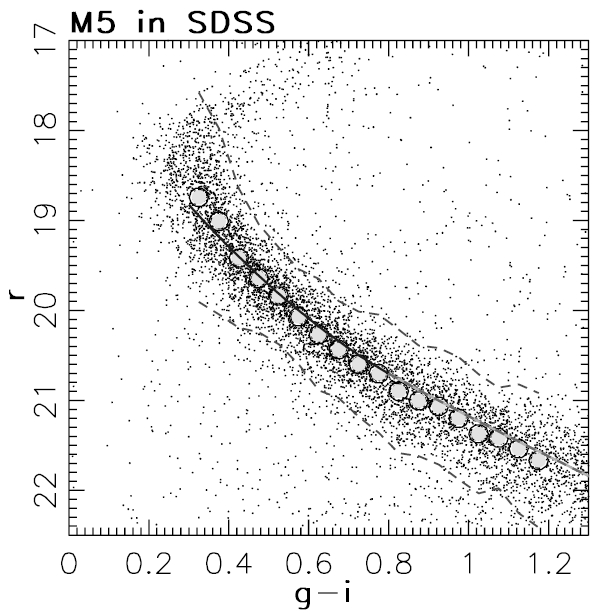
\includegraphics{figures/M5_cmd1.jpg}}
\vskip -0.2in
\scalebox{0.5}{\hskip -2.1in 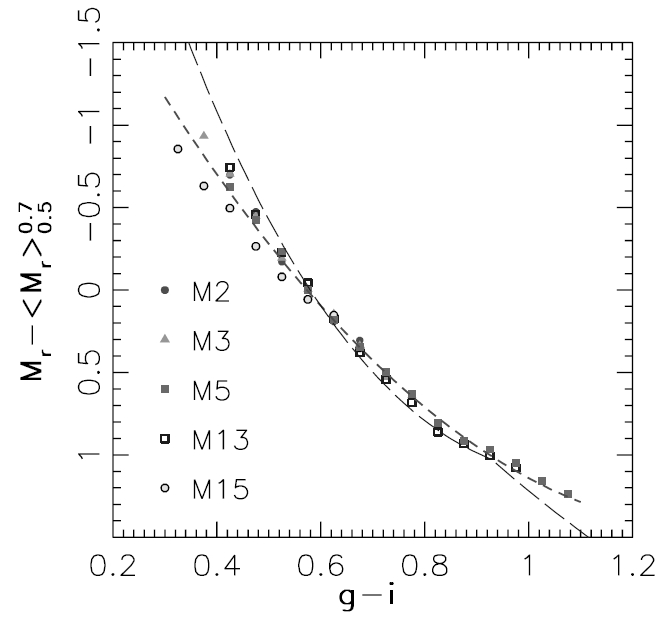
\includegraphics{figures/GCs_cmd1.jpg}}

\end{center}
\end{minipage}

\begin{minipage}[t]{16cm}
\begin{center}
\vskip -1in
{\large \color{red} Photometric Parallax Calibration}
\end{center}


\begin{itemize}
\item {\color{blue} Using a large sample of globular clusters, we can calibrate 
      $M_r(g-i,[Fe/H])$, and then apply it to field stars to get their distances.}
\item {\bf Top Left:} an example of a globular cluster (M5) as observed by
       SDSS; the line is a polynomial fit to the median main sequence (large 
       circles):
\begin{equation}
       M_r = M_r^{0.6} -2.85 + 6.29 \, (g-i) -2.30 \, (g-i)^2  \nonumber
\end{equation}
where $M_r^{0.6}$ is the median absolute magnitude for stars 
with $0.5<g-i<0.7$. 
\item {\bf Bottom Left:} this is a good fit to a number of globular 
  clusters observed by SDSS, showing that the main effect of metallicity
  is to slide the main sequence vertically (i.e. along luminosity axis,
  changing $M_r^{0.6}$), without much effect on its {\it shape}.
\end{itemize}

\end{minipage}}
\vfill 
\end{slide}
%--------------------------------------------------------------------------------------------


%------------------------------------------------------------------------------
% TWO-SIDED PAGE 
\begin{slide}

\hbox to \hsize{
\begin{minipage}[t]{8cm}
\begin{center}
\vskip -0.8in
\scalebox{0.5}{\hskip -1.8in 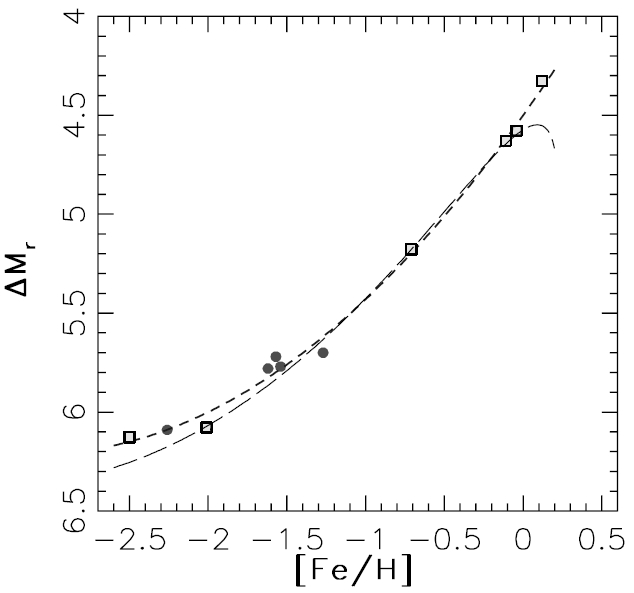
\includegraphics{figures/GCs_FeHshift.jpg}}
\vskip 0.1in
\scalebox{0.5}{\hskip -2.1in 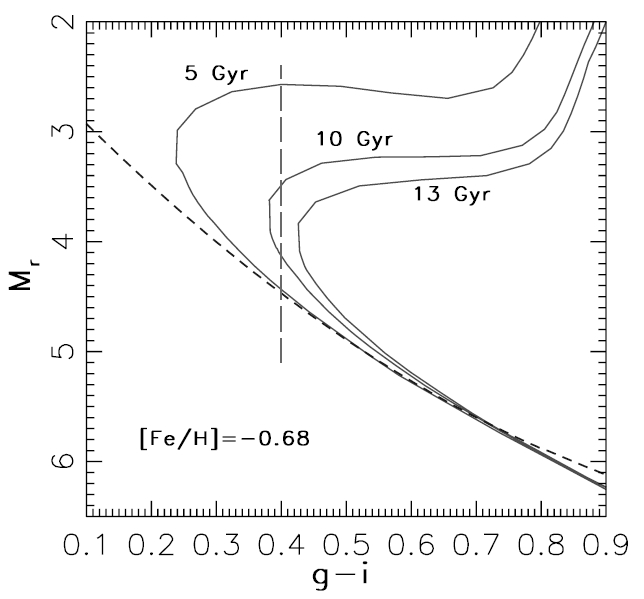
\includegraphics{figures/GCs_age.jpg}}

\end{center}
\end{minipage}

\begin{minipage}[t]{16cm}
\begin{center}
\vskip -1in
{\large \color{red} Photometric Parallax Calibration}
\end{center}


\begin{itemize}
\item {\color{blue} The position of the main sequence depends on [Fe/H]}
\item {\bf Top Left:} calibration (short-dashed) based on SDSS data (dots) and VandenBerg 
       \& Cleam (2003; squares). The shift is huge: $>$1 mag between median 
       halo metallicity ($[Fe/H]=-1.5$) and local disk metallicity  
       ($[Fe/H]=-0.2$).  {\color{blue} Must know [Fe/H] to within 0.2 dex
       to know distances within 10\%!}
\item {\bf Bottom Left:} at a {\bf fixed} [Fe/H], the turn-off depends on 
      the age of a stellar population (based on models!). 
\item For a relation appropriate for age of 10 Gyr (at halo metallicity) see
      eq. A7 in Ivezi\'{c} et al. (2008, ApJ, 684, 287)
\item {\it What about metallicity?}
\end{itemize}

\end{minipage}}
\vfill 
\end{slide}
%--------------------------------------------------------------------------------------------


%------------------------------------------------------------------------------
% TWO-SIDED PAGE 
\begin{slide}

\hbox to \hsize{
\begin{minipage}[t]{8cm}
\begin{center}
\vskip -0.8in
\scalebox{0.5}{\hskip -1.8in 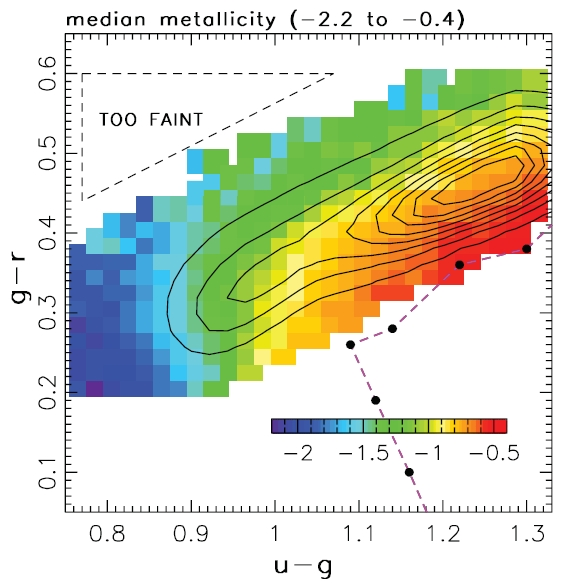
\includegraphics{figures/FeHspecUGR.jpg}}
\vskip 0.2in
\scalebox{0.58}{\hskip -1.9in \includegraphics{figures/FeHphotoVSspec.jpg}}

\end{center}
\end{minipage}

\begin{minipage}[t]{16cm}
\begin{center}
\vskip -1in
{\large \color{red} Photometric Metallicity Calibration}
\end{center}

\begin{itemize}
\item {\color{blue} At a fixed effective temperature, the amount of 
       UV flux ($\lambda<4000 \AA$) for F/G main-sequence stars is very 
       sensitive to metallicity (Wallerstein 1962)}
\item {\bf Top Left:} the dependence of spectroscopic metallicity 
      (using 60,000 SDSS stellar spectra) on the position in the $g-r$ vs. 
       $u-g$ color-color diagram 
\item {\bf Bottom Left:} the correlation between photometric metallicity,
      estimated using a two-dimensional third-order polynomial fit to the
      map shown in the top left panel, and spectroscopic metallicity; 
      the individual values agree with an rms of 0.26 dex (includes errors
      from both methods)
\item {\color{blue} For stars with $0.2<g-i<0.8$, [Fe/H] can be estimated 
      if the $u$ band photometry (or $U$ in Johnson system) is available.}
\end{itemize}

\end{minipage}}
\vfill 
\end{slide}
%--------------------------------------------------------------------------------------------



%------------------------------------------------------------------------------
% TWO-SIDED PAGE 
\begin{slide}

\hbox to \hsize{
\begin{minipage}[t]{0cm}
\begin{center}
%\vskip 0.2in
%\scalebox{0.58}{\hskip -1.9in \includegraphics{FeHphotoVSspec.jpg}}

\end{center}
\end{minipage}

\begin{minipage}[t]{24cm}
\begin{center}
\vskip -1in
{\large \color{red} How good are stellar models?}
\end{center}

\begin{itemize}
\item {\color{blue} Good at predicting absolute magnitudes of main-sequence
    stars to within 0.1-0.2 mag for stars with $T_{eff}>4000$ K.} 
\item An excellent model database: Percival et al. (2009, ApJ, 690, 427)
\item {\bf Bottom:} fig. 5 from An et al. (2009): lines are YREC+MARCS
           models for age of 12.6 Gyr; bulls-eye symbol marks the Sun 
\end{itemize}
\vskip 0.1in
\scalebox{0.8}{\hskip 0.1in 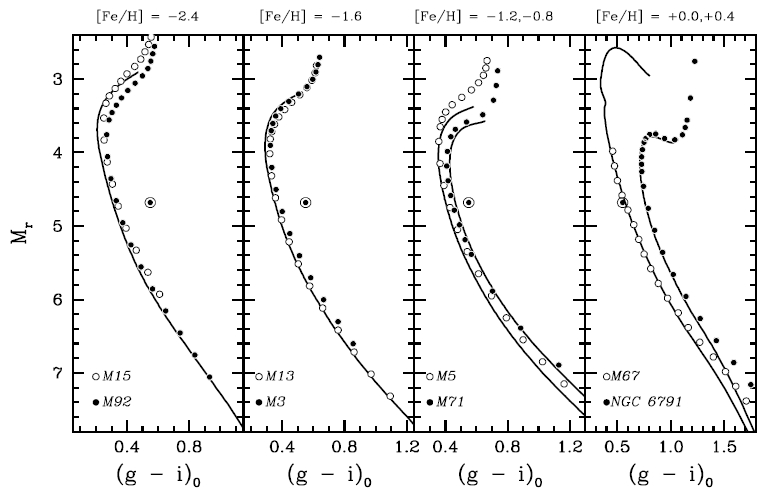
\includegraphics{figures/An09_fig6.jpg}}

\end{minipage}}
\vfill 
\end{slide}
%--------------------------------------------------------------------------------------------


%------------------------------------------------------------------------------
% TWO-SIDED PAGE 
\begin{slide}

\hbox to \hsize{
\begin{minipage}[t]{12cm}
\begin{center}
\vskip -0.8in
\scalebox{1.07}{\hskip -0.8in 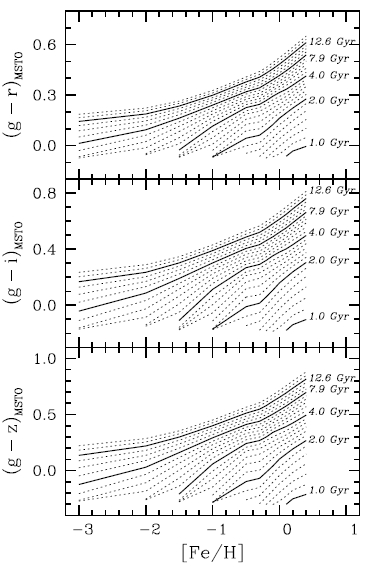
\includegraphics{figures/An09_fig28.jpg}}
%\vskip 0.2in
%\scalebox{0.58}{\hskip -1.9in \includegraphics{FeHphotoVSspec.jpg}}

\end{center}
\end{minipage}

\begin{minipage}[t]{12cm}
\begin{center}
\vskip -1in
{\large \color{red} The turn-off color}
\end{center}

\begin{itemize}
\item {\color{blue} At a fixed metallicity, the turn-off color depends on
       age} (the  color-age translation can be obtained from models).
\item {\bf Left:} the dependence of turn-off color on metallicity and   
       age for YREC+MARCS models (fig. 28 from An et al. 2009)
\item For example, at [Fe/H]=0, the turn-off color changes from 
      $g-i=-0.2$ to $g-i=0.6$ as the age increases from 1 Gyr to 10 Gyr
\item {\color{red} For age$\sim$10 Gyr, the change of color with age
      is very small for all [Fe/H].} The gradient is about 0.02 mag/Gyr:
      requires {\bf exquisite photometry!}  
\end{itemize}

\end{minipage}}
\vfill 
\end{slide}
%--------------------------------------------------------------------------------------------



%------------------------------------------------------------------------------
% TWO-SIDED PAGE 
\begin{slide}

\hbox to \hsize{
\begin{minipage}[t]{10cm}
\begin{center}
\vskip -0.8in
\scalebox{0.65}{\hskip -1.4in 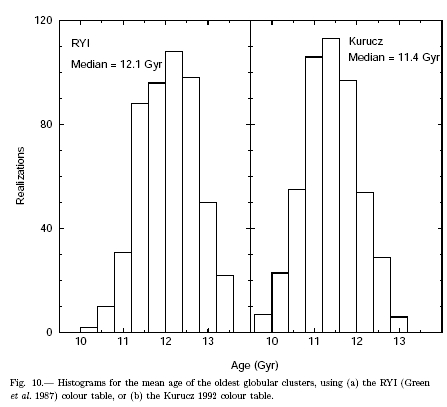
\includegraphics{figures/Chaboyer1.jpg}}
%\vskip -0.007in

An example of systematic effect: (unknown) He abundance
\scalebox{0.60}{\hskip -1.8in 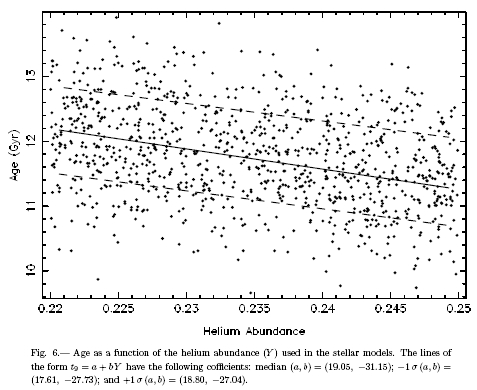
\includegraphics{figures/Chaboyer2.jpg}}

\end{center}
\end{minipage}

\begin{minipage}[t]{13cm}
\begin{center}
\vskip -1in
{\large \color{red} Other Age Determination Methods }
\end{center}


\begin{itemize}
\item {\color{blue} Globular cluster absolute ages provide a strong 
   constraint on the age of the Universe;} however, the 
   simultaneous effects of metallicity, distance, ISM extinction, 
   He abundance, and various model parameters such as mixing length 
   (see Chaboyer et al.; astro-ph/9706128), make age estimates
   uncertain by about 25\% (Jimenez 1998, PNAS 95, 13) 
\item Can we determine age and metallicity using stars that are 
   not on main sequence? Independently of ISM extinction
   correction and distance scale? 
\end{itemize}

\end{minipage}}
\vfill 
\end{slide}
%--------------------------------------------------------------------------------------------


%------------------------------------------------------------------------------
% TWO-SIDED PAGE 
\begin{slide}

\hbox to \hsize{
\begin{minipage}[t]{11cm}
\begin{center}
\vskip -0.8in
\scalebox{0.55}{\hskip -1.7in 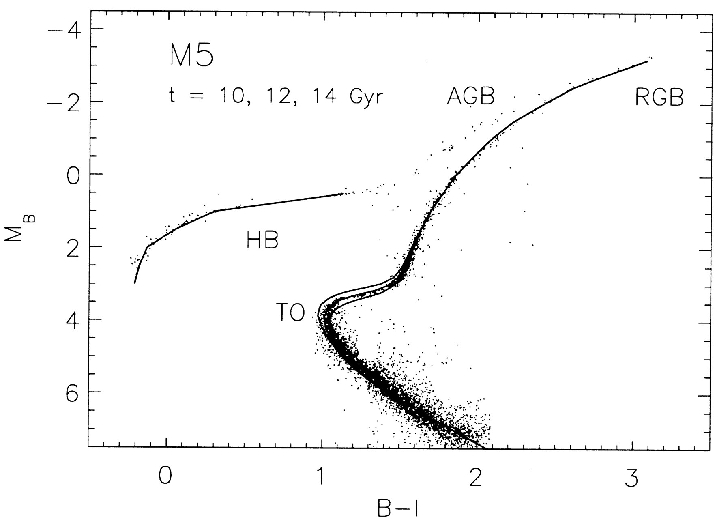
\includegraphics{figures/Jimenez1.jpg}}
%\vskip -0.007in

A comparison of errors for different methods (Jimenez 1998):

\scalebox{0.40}{\hskip -2.3in 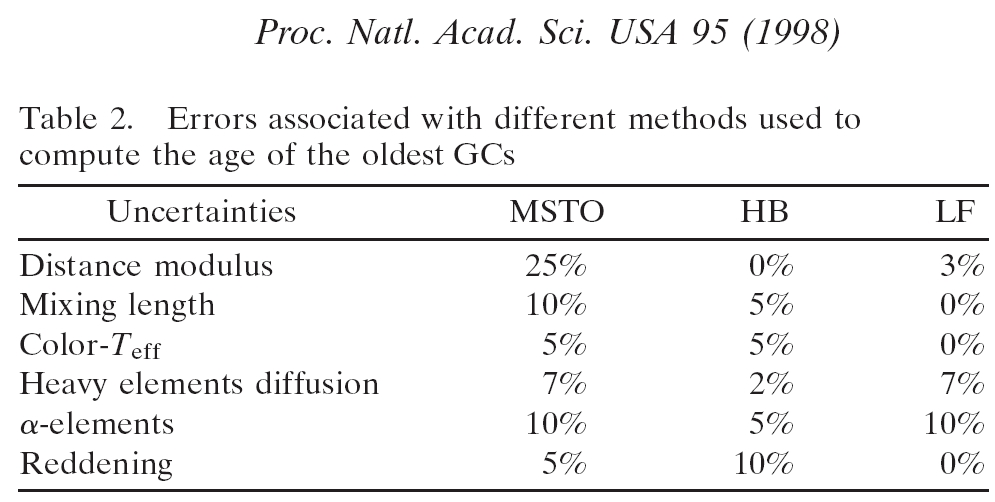
\includegraphics{figures/Jimenez2.jpg}}

\end{center}
\end{minipage}

\begin{minipage}[t]{13cm}
\begin{center}
\vskip -1in
{\large \color{red} Other Age Determination Methods }
\end{center}


\begin{itemize}
\item Can we determine age and metallicity using stars that are 
   not on main sequence? Independently of ISM extinction
   correction and distance scale? 
\item {\color{blue} There are several other methods:} 
   \begin{enumerate}
      \item $\Delta V$ method: measure the magnitude difference between
             the Horizontal Branch and the subgiant branch (Iben \& Renzini 1984);
             about 0.1 mag/Gyr (but also depends on FeH, about 0.2 mag/dex)
      \item Morphology of the Horizontal Branch (Jimenez 1998)
      \item Luminosity Function \\ (Jimenez 1998)
   \end{enumerate}
\end{itemize}

\end{minipage}}
\vfill 
\end{slide}
%--------------------------------------------------------------------------------------------



%------------------------------------------------------------------------------
% TWO-SIDED PAGE 
\begin{slide}

\hbox to \hsize{
\begin{minipage}[t]{6cm}
\begin{center}

\vskip 1.1in
\scalebox{0.7}{\hskip -1.3in 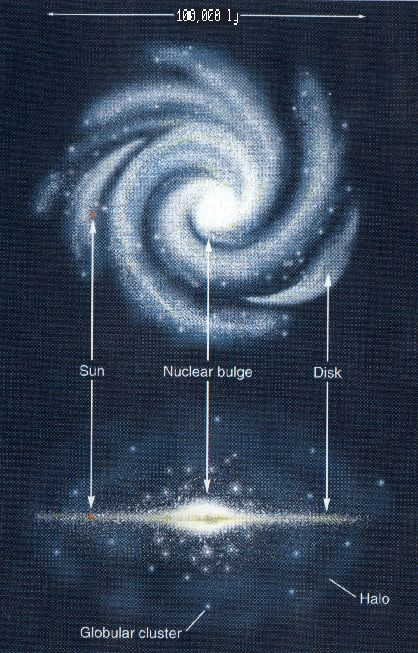
\includegraphics{figures/mw.jpg}}


\end{center}
\end{minipage}

\begin{minipage}[t]{17cm}
\begin{center}
\vskip -1in
{\large \color{red} Properties of GC Population}
\end{center}


\begin{itemize}
\item
{\color{blue} Halo GCs claim to fame: Shapley used their distribution to
demonstrate that the Sun is not in the center of the Milky Way} 
\end{itemize}

\vskip 1in
\scalebox{0.7}{\hskip 1.3in 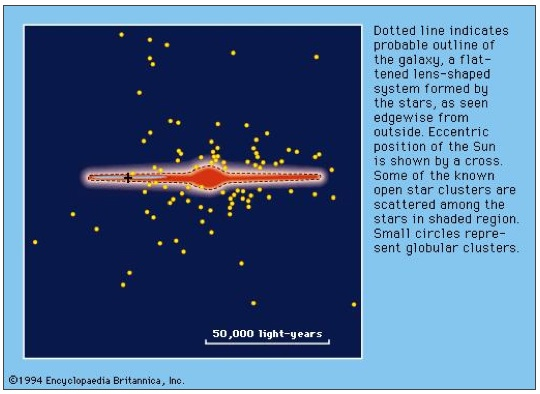
\includegraphics{figures/gc_galaxy.jpg}} 

\end{minipage}}
\vfill 
\end{slide}
%--------------------------------------------------------------------------------------------



%------------------------------------------------------------------------------
% TWO-SIDED PAGE 
\begin{slide}

\hbox to \hsize{
\begin{minipage}[t]{6cm}
\begin{center}
The age vs. metallicity distribution of globular clusters from
Percival \& Solaris. 

\vskip 0.3in
\scalebox{0.5}{\hskip -2.3in 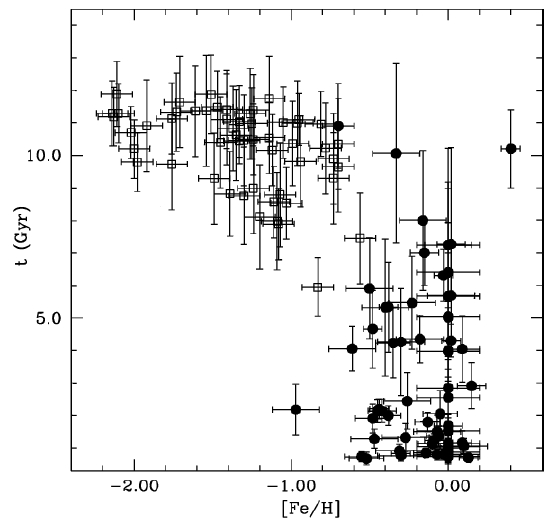
\includegraphics{figures/GC_FeH.jpg}}


\end{center}
\end{minipage}

\begin{minipage}[t]{17cm}
\begin{center}
\vskip -1in
{\large \color{red} Properties of GC Population}
\end{center}


\begin{itemize}
\item
Halo GCs claim to fame: Shapley used their distribution to
demonstrate that the Sun is not in the center of the Milky Way
\item {\color{blue} Most globular clusters are metal-poor}, and thus resemble halo stars. 
Their spatial distribution is also halo-like: roughly spherically distributed,
and at distances of tens of kpc from the galactic center. Kinematics are
similar to halo stars: randomly oriented eccentric orbits. 
\item 
{\color{blue} About 20\% of GCs have higher metallicities ($-1 < [Fe/H] < 0$)} and are
found within 1-2 kpc from the galactic plane. Their distribution and 
kinematics are very similar to thick disk.
\item
These differences are probably due to processes that happened early in the
history of the Milky Way. It is likely that ``thick disk clusters'' formed
after halo clusters. 
\end{itemize}

\end{minipage}}
\vfill 
\end{slide}
%--------------------------------------------------------------------------------------------


%------------------------------------------------------------------------------
% TWO-SIDED PAGE 
\begin{slide}

\hbox to \hsize{
\begin{minipage}[t]{12cm}
\begin{center}

\vskip 0.3in
\scalebox{0.9}{\hskip -1.1in 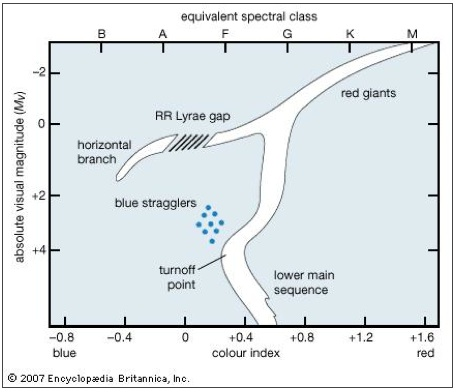
\includegraphics{figures/gc_hr.jpg}}


\end{center}
\end{minipage}

\begin{minipage}[t]{11cm}
\begin{center}
\vskip -1in
{\large \color{red} Properties of GC Population}
\end{center}


\begin{itemize}
\item
Standard modern compilation of globular cluster properties (n=157): 
Harris, W.E. 1996, {\it A Catalog of Parameters for Globular Clusters in the Milky Way},
Astronomical Journal, 112, 1487  (updated in 2010) 
\item Note the existance of the so-called {\it blue straggler} population in the H-R
diagram (left): it shouldn't exist given the cluster turn-off age; it could be the result 
of stellar collisions and mergers 
\end{itemize}

\end{minipage}}
\vfill 
\end{slide}
%--------------------------------------------------------------------------------------------







%------------------------------------------------------------------------------
\end{document}


